% $Id: master_thesis.tex,v 1.4 2004/01/29 08:52:25 yoshi Exp $
% 使う環境に合わせて,以下のどちらかをコメントアウト
%\documentstyle[12pt]{j-report}  % jLaTeX
\documentclass[a4paper,twoside,12pt,uplatex]{jsreport}    % LaTeX2e
\usepackage{multicol}
\usepackage{epsf}
\usepackage[dvipdfmx]{graphicx}
\usepackage{boxedminipage}
\usepackage{epsfig}
\usepackage{amsmath}
\usepackage{amssymb}
\usepackage{ascmac}
\usepackage{enumerate}
\usepackage{xurl}
\usepackage{multirow}
%\usepackage{subfigure}
\usepackage{subcaption}
\usepackage{footnote}
\usepackage[japanese,english]{babel}
\usepackage{siunitx}
\usepackage{amsmath,amssymb,amsthm}% 数式関連のパッケージ
\usepackage{mathtools}
\usepackage[dvipdfmx,hypertexnames=false,setpagesize=false]{hyperref}
\usepackage{pxjahyper}
\usepackage{cleveref}
\usepackage{tabularx}
\usepackage{algorithm}
\usepackage{algpseudocode}
\let\globcount\newcount
\usepackage{autonum}
\usepackage{lscape}
\usepackage{textcomp}

\usepackage{array,etoolbox}
\preto\tabular{\setcounter{magicrownumbers}{0}}
\newcounter{magicrownumbers}
\def\rownumber{}

\crefname{equation}{式}{式}% {環境名}{単数形}{複数形} \crefで引くときの表示
\crefname{figure}{図}{図}% {環境名}{単数形}{複数形} \crefで引くときの表示
\crefname{table}{表}{表}% {環境名}{単数形}{複数形} \crefで引くときの表示
\crefname{algorithm}{Algorithm}{Algorithm}

\crefname{chapter}{第}{第}
\creflabelformat{chapter}{#2#1章#3}
\crefname{section}{第}{第}
\creflabelformat{section}{#2#1節#3}
\crefname{subsection}{第}{第}
\creflabelformat{subsection}{#2#1小節#3}

\theoremstyle{definition}% 日本語用.定理とか斜体にならないようにする
\newtheorem{theorem}{定理}
\crefname{theorem}{定理}{定理}
\newtheorem{lemma}{補題}
\crefname{lemma}{補題}{補題}
\newtheorem{corollary}{系}
\crefname{corollary}{系}{系}
\newtheorem*{proof*}{証明}
\crefname{proof*}{証明}{証明}
\newtheorem{assumption}{仮定}
\crefname{assumption}{仮定}{仮定}
\newtheorem{definition}{定義}
\crefname{definition}{定義}{定義}
\newtheorem{remark}{注意}
\crefname{remark}{注意}{注意}
\newtheorem{proposition}{命題}
\crefname{proposition}{命題}{命題}


\newcommand{\crefpairconjunction}{と}
\newcommand{\crefrangeconjunction}{から}
\newcommand{\crefmiddleconjunction}{,}
\newcommand{\creflastconjunction}{,および}

\captionsetup*[table]{position=top}
\captionsetup*[subtable]{position=top}
\captionsetup*[figure]{position=bottom}
\captionsetup*[subfigure]{position=bottom}


% macro: to explain a line of algorithm figure. #1 is "line number". #2 is "process description"
\def\line#1#2{\hbox{\hbox to 1.5zw{#1:\hfil} #2}}
\def\ub#1{\underline{\bf #1}}

\newenvironment{sourcecode}%
{\begingroup
 \vspace{\baselineskip}
 \vspace{-10.5pt}
 \hrule % height 0.5pt
 \vspace{10.5pt}
 \setlength{\baselineskip}{10pt}
 \footnotesize}%
{
 %\vspace{-10.5pt}
 \vspace{10.5pt}
 \hrule % height 0.5pt
 \vspace{10.5pt}
 \endgroup}

\newenvironment{sourcecode2}%
{\begingroup
 \vspace{\baselineskip}
 \vspace{-10.5pt}
% \hrule % height 0.5pt
% \vspace{10.5pt}
 \setlength{\baselineskip}{10pt}
 \begin{quote}\small}%
{\end{quote}
% \vspace{-10.5pt}
% \hrule % height 0.5pt
 \vspace{10.5pt}
 \endgroup}


% ページサイズを指定 (LaTeX2eと相性がいいかも?)
%\oddsidemargin -10 pt      %   Left margin on odd-numbered pages.
%\evensidemargin 10 pt      %   Left margin on even-numbered pages.
%\marginparwidth 1 in       %   Width of marginal notes.
%\oddsidemargin 0 in      %   Note that \oddsidemargin = \evensidemargin
%\evensidemargin 0 in
%\marginparwidth 0.75 in
%\textwidth 6.375 true in % Width of text line.
%\textheight=620pt

%\input{MyEnvironment.tex}
%\input{Pagestyle.tex}
%\renewcommand{\bibname}{参考文献}

%========================================================================%
%========================================================================%
%========================================================================%

\begin{document}

% ここで行間を調整
\baselineskip 22pt
%\baselinestretch{3.0}

%======  タイトルと要旨  ================================================%
\begin{titlepage}
  \Large
  %\vspace*{9mm}
  \begin{center}
   %%%%%%%%%%% タイトル,氏名,所属,指導教員%%%%%%%%%%%%%%
   {\LARGE     %%% for 12pt
      SNSに投稿された音声を含む偽情報\\に対応した早期検出手法の提案
    }
  \end{center}
  \vspace{60mm}
  \centerline{\bf 栁 裕太}
  \vspace{20mm}
  \centerline{電気通信大学大学院情報理工学研究科}
  \centerline{博士(工学)の学位申請論文}
  \vspace{25mm}
  \centerline{\large 2024年12月}


  %%%%%%%%% 博士論文審査委員会
  \cleardoublepage
  \begin{center}
   %%%%%%%%%%% タイトル,氏名,所属,指導教員%%%%%%%%%%%%%%
   {\LARGE     %%% for 12pt
      SNSに投稿された音声を含む偽情報\\に対応した早期検出手法の提案
    }
  \end{center}
  \vspace{60mm}
  \hspace{50mm}博士論文審査委員会\\
  %\hspace{60mm}主査 \hspace{6mm} 大須賀 昭彦 \hspace{3mm} 教授\\
  \hspace{60mm}主査 \hspace{6mm} 田原 康之\hspace{3mm} 准教授\\
  \hspace{60mm}委員 \hspace{6mm} 折原 良平\hspace{3mm} 連携教授\\
  \hspace{60mm}委員 \hspace{6mm} 内海 彰 \hspace{6mm} 教授\\
  \hspace{60mm}委員 \hspace{6mm} 羽田 陽一\hspace{3mm} 教授\\
  \hspace{60mm}委員 \hspace{6mm} 稲葉 通将\hspace{3mm} 准教授\\
  \thispagestyle{empty}
  %%%%%%%%%% 著者権 %%%%%%%%%%%%%%%%%%%%%%%%%%%%%%%%%%%%%
  \cleardoublepage
  \vspace*{70mm}
  \centerline{\LARGE 著作権所有者}
  \vspace{20mm}
  \centerline{\bf 栁 裕太}
  \vspace{10mm}
  \centerline{\large 2024}
  \thispagestyle{empty}
\end{titlepage}
\thispagestyle{empty}
\cleardoublepage
\selectlanguage{english} 
\thispagestyle{plain}
\begin{center}
    \Large
    \textbf{Towards a Safer Social Media: AI-Powered Detection of Disinformation in Text and Audio}
        
    \vspace{0.4cm}
    \textbf{Yuta Yanagi}
       
    \vspace{0.9cm}
    \textbf{Abstract}
   
\end{center}
%\begin{center}
%    \vspace{5mm}
%        {\Large \bf Proposal of Artificial Intelligence Models for\\Detecting Disinformation on Diversified Social Media}\\
%    \vspace{10mm}
%    Yuta Yanagi
%\end{center} 
%\begin{abstract}
This doctoral dissertation examines innovative methodologies for identifying disinformation, 
with a particular emphasis on the evolving challenges posed by synthetic audio in social media. 
Two principal methodologies are put forth to address the shortcomings of existing text-centric approaches and the accelerated advancement of audio synthesis technology.
The initial method employs comment-generation techniques to augment the detection of disinformation on text-based social media platforms. 
The Grover model serves as a foundation for developing a system that generates comments based on news articles and existing comments, thereby simulating post-diffusion scenarios. 
The experiments demonstrate that the incorporation of generated comments enhances the recall of disinformation detection, 
thus enabling the identification of such content even when comment availability is limited.
The second method addresses the detection of synthetic audio conveying disinformation, 
with a particular focus on both the speech waveform and the content. 
A novel framework combines waveform analysis using established spoofing detection models (RawNet2, RawBoost, SSL-Antispoofing)
with content analysis leveraging text embeddings from the MuMiN dataset. 
This approach demonstrates a notable enhancement in the classification of synthetic voices propagating disinformation when compared to a strategy that relies exclusively on waveform analysis.

%\end{abstract}

%Recently, it is expected that personal information stored by different service providers are combined securely and it will create a new service. However, there is a risk that a specific user record can be identified by the combined personal information, and the user's sensitive information is revealed. Also, the personal information collected by the service provider must not be disclosed to other service providers because of security and privacy issues. Thus, related researches have been conducted on distributed anonymization methods, which combine the personal information stored by the providers and sanitize it to ensure a policy of anonymity with the minimum disclosure.

%However, in those researches, if sets of the users among the providers are different, a problem occurs that the users' presence in either provider may be revealed. Therefore, this paper proposes a new indicator, named {\it $\delta$-site-presence}, which represents the probability of the users' presence being revealed. Also, this paper proposes an improved distributed anonymization protocol which satisfies the proposed indicator. This protocol uses dummy users who do not exist in the provider. The providers treat the dummy users as if they actually exist. By using the dummy users, it can anonymize the personal information without disclosing the users' presence.

%We evaluate the security of the proposed protocol and proof that the protocol does not disclose any sensitive information. In addition, we evaluate the processing and communication cost of the protocol. The evaluation results show that the cost of the proposed protocol is not much higher than that of the existing protocols. 

%Moreover, we evaluate the utility of the proposed protocol with U.S. Census data and health data. Our evaluation results show that the proposed protocol can anonymize them with lower information loss than the existing distributed anonymization method.

%It is expected that our method combine not only census data and health data but also several types of the personal information and there is a possibility that a new service will be created.
%\\

\thispagestyle{plain}
\cleardoublepage
%
%
%%%%%%%% 和文の概要 %%%%%%%%%%%%

\begin{center}
    \Large
    \textbf{SNS に投稿された音声を含む偽情報に対応した早期検出手法の提案}
        
    \vspace{0.4cm}
    \textbf{栁 裕太}
       
    \vspace{0.9cm}
    \textbf{概要}
   
\end{center}

\selectlanguage{japanese} 
%\begin{abstract}
%背景
ソーシャル・ネットワーキング・サービス(SNS)の発展によって誰もが情報を共有できるようになった反面、悪意によって意図的に作成された偽情報が多くの社会問題を引き起こしている。
人手による偽情報の検出には時間がかかるため、人工知能によって自動で検出する手法が求められている。
その中で、利用者の反応を考慮した研究も提案されているが、早期検出を目指した場合に十分な反応を得ることができないという課題がある。
また、新しい情報生成技術の登場や広く使われるSNSの変化によって、検出において必要な要求が大きく広がりつつある。
%よって、文章を中心とした既存の手法では検出性能を長い期間維持しにくいほか、新しい媒体を使用したSNSへの適用も難しい。
具体的には、文章や画像といった情報の形式も、動画や音声といった新たな形式への対応が求められている。
特に音声では、手軽に自然な音声を得られるようになったため、音声を使った偽情報が急増しているにも関わらず、
十分に有効な検出手法が提案されていない。
そこで本論文では現状特に対策が必要な、偽情報を喧伝するなりすまし音声に対する新たな検出手法を2つ提案する。
1つはどの形式の情報・投稿に対しても自然言語として投稿されるコメントを扱う手法であり、もう1つは偽情報を喧伝するなりすまし音声に対して合成/本人と事実/虚偽という2つの観点から検出する手法である。

%実験1
%%目的
音声を含めたどの情報形式へ対応可能な手法として、コメントの生成による検出の補助を目指した。
事実に基づく情報に比べて、偽情報のコメントは批判的な内容になりやすいという点が、先行研究によって明かされている。
よって記事に加えて寄せられたコメントを使った検出が有用である反面、
早期検出においては多数のコメントの活用が難しい部分に着目した。
そこで本研究は早期検出と高精度の両立を目指して、記事に対するコメントを生成して拡散後の状況を擬似的に作り、偽情報検出を補助する手法を提案する。
%手法
提案手法は記事の本文と3件のコメントからコメントを生成する学習を行い、記事の内容に対してどのようなコメントが寄せられたか把握させる。
%この手法の開発にあたって、偽情報を生成する既存手法を改変して実装した。
%実験
%\newpage
英文記事とコメントのデータセットを使用した実験では、学習させた手法に対して本文と2件のコメントから追加で1件コメントを生成させた。
検出性能を調べるため、生成コメントを加えたセットを別の偽情報検出モデルに入力して性能に変化があったか調べた。
比較対象として、記事本文のみで検出を行った場合と、本文と実在コメント2件のみで検出を行った場合を用意した。
提案手法の芸能関連の記事に対する再現率(Recall)は0.695と全体で最も高い結果を示し、より多くの偽情報を検出した。
一方で適合率(Precision)に改善の余地を残しているものの、生成コメントの追加によって検出結果がFakeに覆った割合が48\%と、生成コメントの追加による効果がみられた。
また、政治関連の記事に対してはいずれの指標においても生成コメントを追加しない場合の結果を上回った。
% 既存手法で不足している指摘
% なぜこの手法を開発することにしたか?という部分は確実に聞かれる
% コメント生成→媒体に左右されにくい+何らかのポイントを追加したい
% 音声→現状で手薄
% 全体図で手薄な部分の指摘と全体に適用可能な形式
% サーベイ論文で既にある指摘なら引用して説得力補強
% もう一息説得力がほしい
% 動画対象はどこまでできている?

%\newpage
%実験2
%%目的
また、合成音声が話す偽情報に対して「誰が」「何を」話しているかという2視点から検出を行う手法を提案する。
新たなSNSとして文章や画像以外を扱う形式が出現していることと、生成技術の発展で任意の人物の音声を容易に再現できるようになっている点
%、そして合成技術の発展によって音声波形のみから検出する手法の性能維持が難しくなっている点
から、本研究では音声を対象とした。
%手法
既存の合成音声検出手法の多くは生体認証システムを想定した形式であるため、音声波形を分析する形が中心だった。
しかしながら、SNS上にて合成音声による偽情報を検出したい場合、内容の疑わしさも考慮に入れる必要がある。
よって本研究は虚偽の主張を行うなりすまし音声の検出を目標に、発話内容と音声波形の両面から検出を行う手法を提案する.
提案手法では、既存手法と同じく音声波形を直接入力とする部分と、
発話内容の信憑性を評価するための文章埋め込みを入力とする部分からなる.
%実験
SNS上に投稿された文章を読み上げる合成音声を使った実験では、
音声波形のみを考慮した手法では等価エラー率が50.7\%とランダム選択に近しい結果を示したことに対して、提案手法では17.6\%と改善がみられた。

%結論
これらの提案手法を用いることによって,
疑わしい主張を行う音声に対してコメントの生成という新しい形式の真偽判断材料を提供するとともに,
文章による記事に限らず,波形と内容の両面から真偽確認を可能にすることで,
SNS利用の安全性向上への貢献が期待できる.
%
%\end{abstract}

\cleardoublepage

\pagenumbering{roman}
\setcounter{page}{1}
\pagestyle{plain}
%======  目次の生成  ====================================================%
\tableofcontents
\listoffigures
\listoftables
\cleardoublepage

%\listofprograms

%\newpage
\pagestyle{headings}
\pagenumbering{arabic}
\setcounter{page}{1}

\cleardoublepage
\chapter{はじめに}
\label{ch:introduction}
現代において,ニュースを始めとする情報入手と拡散が簡単にできるSNS(ソーシャルメディア)は生活の重要な一部となった.
SNSは現在$\mathbb{X}$(旧Twitter、以後Twitterと表記)をはじめFacebook, Instagram, YouTube, TikTokと多くのプラットフォーム上に多様な情報が拡散されている。
しかし、中には信憑性に乏しい情報が含まれており,特に悪意によって読者を騙して誤った風説を流布するために作られた情報であるフェイクニュース及び偽情報が社会問題となっている.
%フェイクニュースの国際的にコンセンサスが取れた定義はないが,``Fake news''という語は既に19世紀の文献に使われているという報告が英英辞典出版会社であるMerriam-Webstarから指摘されている\cite{merriam-webster}.
%また同時に辞書に載せない理由としてフェイクニュースという語が自明の意味をもつためとも指摘されている\cite{merriam-webster}.
本研究はこれまでの研究\cite{Shu:2017:FND:3137597.3137600,Ruchansky:2017:CHD:3132847.3132877,Wang:2018:EEA:3219819.3219903}に倣い,意図的に作成され,明確に誤りであると確認できる情報を偽情報と定義し、検出対象とする.

偽情報の実例として,近年は新型コロナウイルス感染症(COVID-19)にまつわる誤った風説がSNS上で広く流布された.
WHO事務局長はこの問題を``インフォデミック''と呼び,偽情報はウイルスそのものよりも早く簡単に拡散されると警戒を呼びかけている\cite{ZAROCOSTAS2020676}.
また,偽情報によってオンラインで誤った風説が広がった結果,オフラインの出来事へ大きな影響を与えたこともある.
英国では「第5世代移動通信システム(5G)が健康被害をもたらし,新型コロナウイルス感染症蔓延に寄与している」という偽情報に基づく陰謀論が流布された結果,基地局の設備が壊された\cite{waterson_hern_2020}ほかに作業員が暴行や暴言を受けた\cite{hern_2020}.
以上より,偽情報の拡散によって読者が事実に基づく正しいニュースへのアクセスが難しくなるため、政情不安・暴力・テロリズムを引き起こすことで民主主義の根幹を揺るがす深刻な問題であると世界経済フォーラムの年次報告書は指摘している \cite{mclennan2024global}.

現在,偽情報検出に向けて有識者が事実関係を確認して結果を公表するファクトチェックが行われている.
\begin{figure}[p]
    \centering
    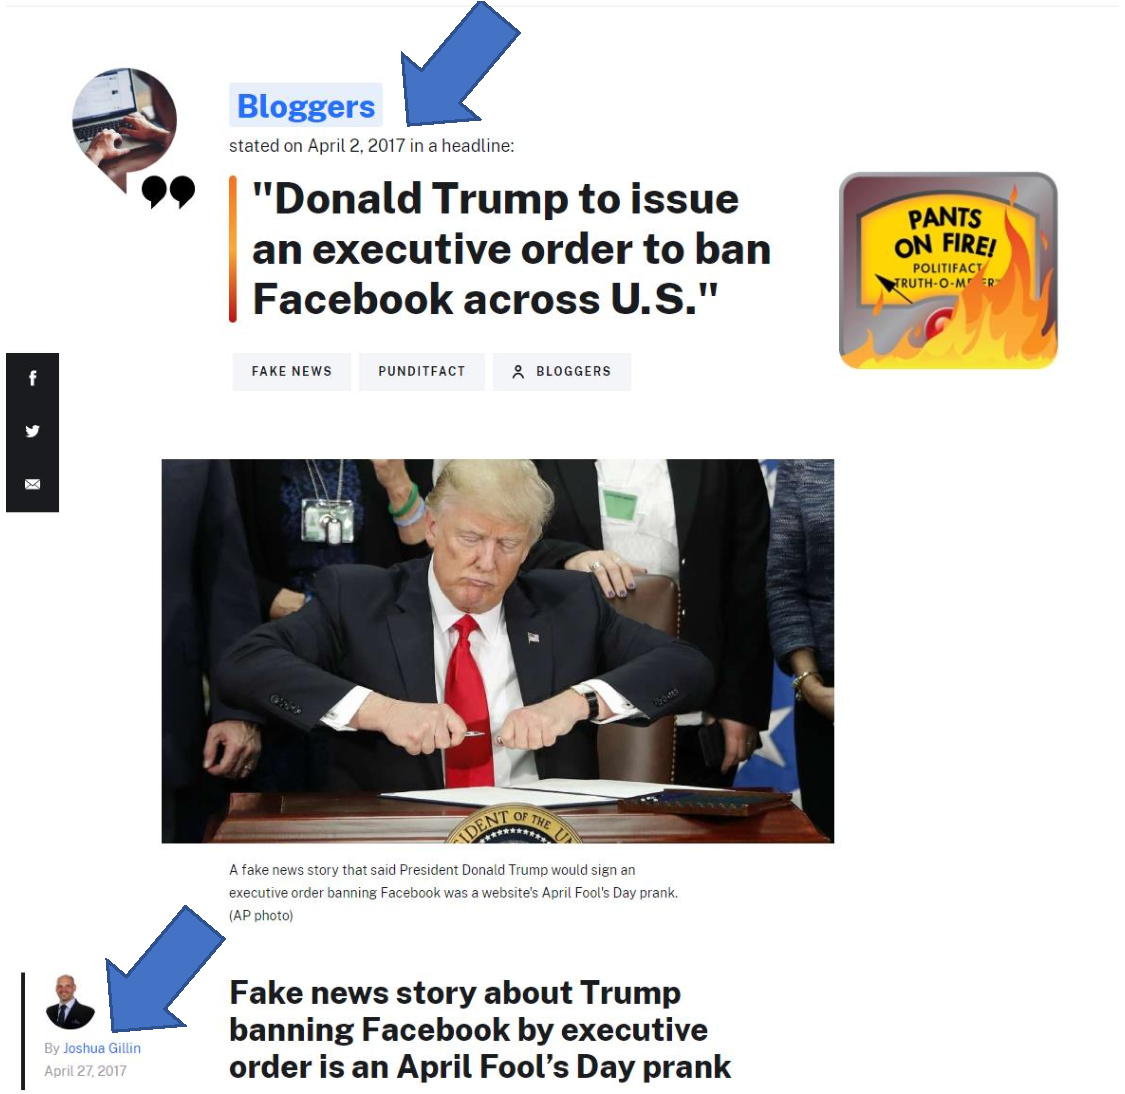
\includegraphics[width=0.8\linewidth]{figures/fact-check.pdf}
    \caption{
        北米で行われたファクトチェックの一例.
        % この情報はエイプリルフールで投稿された虚偽情報としている.
        青矢印は元情報の投稿日時とファクトチェック結果投稿日時を示し,両者には25日もの間隔がある.
        }
    \label{fig:example}
\end{figure}

図\ref{fig:example}はファクトチェックの一例である\cite{gillin_2017}.
この実例のように,ファクトチェックは属人的な作業であることに加えて結果公表まで時間がかかるため,
ファクトチェック結果は偽情報そのものに比べて拡散されにくい.
このため,機械学習によって偽情報を自動で検出する研究が行われている.

自動検出にあたって困難な点として,偽情報は人々を騙すために巧妙なつくりをしていることが挙げられる.
このため,単純なルールベース手法による検出は難しい.
また、現在偽情報をとりまく状況は変化しており、文章に限らず画像・動画・音声など多様な媒体で発信されるようになった。
\cref{tab:modality}は4種の媒体別の流布頻度と既存研究から現在の状況を示している。
文章・画像は流布される頻度が最も高い一方で多くの既存研究が提案されている。
一方で動画は流布される頻度が上昇傾向にあるが、動画の多くは拡散の早い段階で虚偽と検証されて拡散に歯止めがかかりやすい上に、
動画及び映像を検出対象とした研究も多数提案されている。
しかしながら音声は流布される頻度が動画以上に激しい上昇傾向にある。
その上、既存研究の多くはSNSではなく生体認証から発展させた形であるため、現在の偽情報を取り巻く状況への合致が求められている。
% 

\begin{landscape}
\begin{table}[p]
    \centering
    \begin{tabular}{l|c|c|c} \hline
       媒体 & 流布頻度 & 既存研究 & 概説\\ \hline\hline
       文章 & 多い & \cite{yanagi2021classifying,10.1145/3292500.3330935} & 噂を含めれば最も高い頻度で流布されている一方、検出を目指す既存研究も多い \\
       画像 & 多い & \cite{Wang:2018:EEA:3219819.3219903,8919302} & 記事文章と関係ない画像の使用や合成・生成画像を検出対象とした研究が多い \\
       動画 & 緩やかな増加 & \cite{8683164,8668407} & 増加傾向にあるが、その多くは早い段階で虚偽として注意喚起がなされている \\
       \multirow{2}{*}{音声} & \multirow{2}{*}{急激に増加\cite{cox_2023}} & \multirow{2}{*}{\cite{yamagishi21_asvspoof}} & %動画の構成要素としての音声や
       激しい増加に個別の検証が追いついていおらず、\\
       & & & 自動検出する研究もSNSを想定した形は限られる \\ \hline
    \end{tabular}
    \caption{偽情報の媒体別の流布状況及び既存研究に準拠した状況の概説}
    \label{tab:modality}
\end{table}
\end{landscape}

% 媒体を問わず唐突?
本研究では、現状AIによる生成技術の発展に検出が追いついていない偽情報を話す音声の検出も視野に入れ、
媒体を問わず広く検出が行える手法と音声に特化した手法の2種類を提案する。
これにより、急速に変化する偽情報を取り巻く事情に多面的に対処が可能となる。

先行研究では、検出性能の向上において,記事そのものがもつ情報に加えてソーシャルメディア上での反響を示すソーシャルコンテキスト(リツイート・いいね・リプライなど)
を考慮する有効性が指摘されている\cite{Guo:2018:RDH:3269206.3271709}.
しかしながら,ソーシャルコンテキストはユーザの拡散によって生まれるため,この場合も早期の検出には向かない.
これに対して,ニュースに対してソーシャルメディア上で寄せられるコメントで発生しやすい単語を,条件付き変分オートエンコーダ(CVAE)で生成する手法も提案されている\cite{ijcai2018-533}.
この手法は,記事から確率分布とラベルを元に隠し変数を介して生成を行っている.

本研究では、記事と実際に記事に寄せられたコメントから信憑性の学習を行い,記事と限られた数のコメントから別のコメントを予測させた上で真偽を判断するモデルを提案する。
このモデルは,偽情報そのものを生成するモデル\cite{DBLP:journals/corr/abs-1905-12616}を拡張する形で実装することでコメントの生成を実現する.
学習では記事と実際に記事に寄せられたコメントを3件,更に真偽ラベルを入力するが,テスト時は記事に加えて実際に寄せられたコメントは2件に制限し,真偽ラベルは入力しない.

我々は提案モデルの検出性能を実際に投稿された情報をもつデータセットによって検証した結果,生成コメントを加えた影響でより多くの偽情報を検出することに成功した.
また生成コメントの有無で検出傾向を調べたところ,生成コメントの追加によってFakeをRealと誤認する事例が減少したことが確認された.

一方で、近年さらに偽情報の検出を困難にしている点として、音声や動画といったニュース媒体の多様化が挙げられる。
中でも偽情報を話すなりすまし偽音声や偽動画も偽情報問題と同じく、センセーショナルさを持つがゆえにソーシャルメディアで急速に拡散される危険性を持っている。
広く拡散された偽情報動画の例として、2022年にウクライナのゼレンスキー大統領になりすましたものが挙げられる。
\cref{fig:zelensky}はその動画と本人の写真を並べたものである。
\begin{figure}  %TODO: かえる
    \centering
    
\includegraphics[width=0.45\textwidth]{figures/zelensky.png}
    \caption{ウクライナのゼレンスキー大統領が動画で投降を呼びかける音声付きディープフェイク動画 \cite{evon_2022}.}
    \label{fig:zelensky}
\end{figure}
この動画は武器を捨てて投稿するよう呼びかけていたが、事実確認(ファクトチェック)によって虚偽と認められた \cite{Staff_2020}。
他にもアメリカのペロシ前下院議長になりすました動画は2023年に新たに投稿されており、ロイター通信によって虚偽と確認されている \cite{Check_2023}。
このようなディープフェイク映像の対策として、映像そのものの分析 \cite{8683164}やメディアの出自 \cite{8668407}から信憑性を評価して検出を目指した研究が提案されている。
なりすまし音声による虚偽の主張が盛んに投稿された事例もある。
2023年初頭に公開された音声生成AIによって有名人になりすました偽情報がSNSに投稿され、中には人種及び性的少数者に対する差別的なものも含まれていた \cite{cox_2023}。
容易に特定の人物を模した音声を合成する手法には、文章を入力に出力音声を得るText-To-Speech(文章読み上げ、TTS) \cite{klatt1987review}と、他人の音声を入力に対象人物の音声に変換するVoice Conversion(音声変換、VC) \cite{661472}の2種類がある。
\cref{fig:vctts}は2種類の手法によるなりすまし事例を示す模式図である。
本研究では、TTSによって生成された音声を検出対象とした。
これは少ないコストで大量に合成音声を用意できる点から、すべてを人手での確認することが難しく自動で検出する必要が強いためである。
\begin{figure}[p]
\centering
  \begin{minipage}[b]{0.8\linewidth}
    \centering
    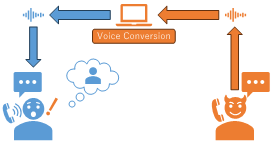
\includegraphics[keepaspectratio, width=0.8\linewidth]{figures/vc.png}
    \subcaption{Voice Conversionによる場合。}
  \end{minipage}
  \begin{minipage}[b]{0.8\linewidth}
    \centering
    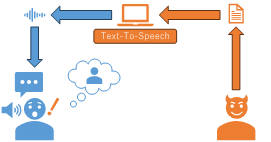
\includegraphics[keepaspectratio, width=0.8\linewidth]{figures/tts.png}
    \subcaption{Text-To-Speechによる場合。}
  \end{minipage}
  \caption{偽音声によるなりすましを示す模式図。(a)のVoice Conversionでは攻撃者の音声が入力であり、(b)のText-To-Speechでは文章が入力であるため攻撃者の音声は含まれない。}
  \label{fig:vctts}
\end{figure}

なりすまし音声による偽情報に対して現在行われている検出手法の多くは、生体認証システムに対する攻撃を念頭に置いたものが中心である。この代表としてASVspoof \cite{7858696,kinnunen17_interspeech,todisco19_interspeech}という共有タスクが2015年から隔年で開催されている。
以前は電話回線や録音再生を想定したシナリオに限られていたが2021年の開催で初めてSNS上での投稿を想定したシナリオが追加された \cite{yamagishi21_asvspoof}。
この取り組みでは同じ文章を人間が読み上げたものと合成音声による2種へ分類を行うモデルを募っている。
読み上げる内容は同じであるため、参加手法は音声波形を直接入力として扱っている\cite{jung20c_interspeech,9746213}。
ASVspoof以外では入力音声から声道を再構築して合成か本物かを判断する手法も提案された \cite{280020}。

これら手法が共通して抱える問題点として、合成側の技術進歩が著しい上に検出手法は攻撃側も利用できるため、生成性能の向上による検出性能の低下が激しい点が挙げられる。
実際に2021年に開催されたASVspoofでは、学習用データは2019年開催のものを流用し、手法の評価には2019年以降に提案された新型生成手法によって生成された音声を使用した。
その結果、学習時の分類性能に比べて評価時の性能が大きく劣化する傾向がみられた \cite{yamagishi21_asvspoof,yu_icmece}。
一方で、問題を起こすなりすまし音声は虚偽の主張を行うものが多いため、
音声内で話される内容を含めて信憑性を評価することは有効と考えられるが、そのような手法はみられない。
今後合成音声の精巧化が進むと、波形そのものの自然さ/クオリティの検証と同時に発話内容そのものを検証する重要性が強まることが予想されている \cite{10208955}。

そこで本研究では、発話内容も考慮に入れてなりすまし音声による偽情報を自動で検出するモデルの構築を目指した。
具体的には、入力音声そのものが合成あるいは本物であるかと、主張内容は疑わしいかそうでないかという2点の観点からなりすまし音声による偽情報の検出を行う。
検出対象として、既存の偽情報データセット \cite{10.1145/3477495.3531744}が持つTwitterツイート群から、
直近提案された中で著名なTTS手法であるVITS \cite{pmlr-v139-kim21f}によって生成した音声データを用意した。
本研究の目的は既存の手法に新たに発話内容を考慮する重要性を示すものであるため、
入力音声そのものを直接入力として扱う手法は既存のものを使用した。
発話内容の考慮には、偽情報データセットの各ツイートから得た文章埋め込みをニューラルネットワークを介して信憑性を評価する独自モデルを用意した。
この結果、音声波形のみを扱う手法では、直近の合成音声手法による偽音声を正確に検出できなかった点に対して,
文章埋め込みに基づく真偽二値分類に由来する入力を追加することによって、検出性能が改善した.


%全体の流れ
本論文の構成は次の通りである.
\cref{ch:background}では,本研究が扱う偽情報に関する背景を実例を交えて記述する.
\cref{ch:rel_res}では,本研究と関連のある研究や取り組みを紹介する.
\cref{ch:gen_com}では,第一の手法として記事に対してコメントを生成して検出を補助する形式及び実験を説明する。
\cref{ch:spc_cnt}では,第ニの手法として発話音声も加味したなりすまし偽音声検出を行う形式及び実験を説明する.
\cref{ch:discussion}では,\cref{ch:gen_com}と\cref{ch:spc_cnt}の実験を併せた全体の考察とともに、手法や結果から浮かび上がった課題についても指摘する.
\cref{ch:conclusion}では,本論文をまとめるとともに,実用化を含めた今後の発展形についていくつかの展開を記載している.
\cleardoublepage
\chapter{背景}
\label{ch:background}
\section{検出対象の定義}
%第\ref{ch:introduction}章の通り,フェイクニュースの国際的にコンセンサスの取れた定義はない.
偽情報に類似した語として、フェイクニュースがある。
フェイクニュースの国際的にコンセンサスの取れた定義はないものの、
英英辞典によっては定義を説明しようという取り組みもあり,コリンズ英英辞典では以下のように定義している\cite{collins_fake}.
\begin{quote}
    false, often sensational, information disseminated under the guise of news reporting
\end{quote}
ここでは,ニュース報道を模したセンセーショナルな虚偽の情報と定義している.
またコリンズ英英辞典は2017年を代表する語として``Fake news''をWord of the Yearに選定している\cite{collins_word}.
一方,同じ出版会社から出されているコウビルド英英辞典では,次のように定義している\cite{collins_fake}.
\begin{quote}
    If you describe information as fake news, you mean that it is false even though it is being reported as news, for example by the media.
\end{quote}
この定義はある記事をフェイクニュースと指摘した場合,例えマスメディアが発信したニュースであろうと虚偽の情報が含まれることを意味するとしている.
コリンズ英英辞典と定義が異なるのは,虚偽の情報が含まれていると指摘したい時に使う状況を想定しているためとみられる.
このように、Fake newsという語は同じ出版会社の英英辞典でも定義にゆらぎがみられる。

%misinformation, disinformation
フェイクニュース(Fake news)と近い意味を持つ言葉としてMis-informationとDis-information, そしてMal-informationがある.
これらの違いに関しては欧州評議会が出版したWardleとDerakhshanによる文書により、以下の\cref{fig:info}の通り真偽性と有害性によって分類されている\cite{wardle2017information}.

\begin{itemize}
    \item \textbf{Dis-information}: 虚偽の情報であり,個人や集団に対して有害な情報.
    \item \textbf{Mis-information}: 虚偽の情報である一方,悪意はなく有害性はない情報.%日本語における「誤報」や「誤情報」の定義に近い.
    \item \textbf{Mal-information}: 事実に基づいた情報であり,個人や集団に有害性を持たせるために用いられる情報.リークやヘイトスピーチなどが含まれる.
\end{itemize}

このうちDis-informationは欧州委員会の報告書でもdisinformationとして以下の通りに定義されている \cite{doi/10.2759/739290}。
初期の定義付けされた場合の単語に対して表記揺れが起きているが、ハイフン無しの表現が一般的となっている。

\begin{quote}
    all forms of false, inaccurate, or misleading information designed, presented and promoted to intentionally cause public harm or for profit
\end{quote}

日本語では、総務省で開催された研究会で disinformation への対訳として「偽情報」と表現している \cite{soumuDisinfo}。
また、2024年現在では政府広報より日本語の偽情報と誤情報の違いとして以下の定義付けがなされている \cite{gov2024}。

\begin{itemize}
    \item 偽情報とは?:
    人を混乱させ惑わすために意図的・意識的に作られたウソ、虚偽の情報
    \item 誤情報とは?:
    勘違いや誤解により拡散された間違った情報
\end{itemize}

本研究では,第\ref{ch:introduction}章の通り検出対象の定義をdisinformation・偽情報に該当するものとする.
また、偽情報の定義としては情報の内容に焦点を当てている点に留意する必要がある。
%また、本研究が検出対象とする情報の範囲から鑑みて、便宜上本論文では検出対象をdisinformation及び偽情報として表記する。

\begin{figure}[p]
    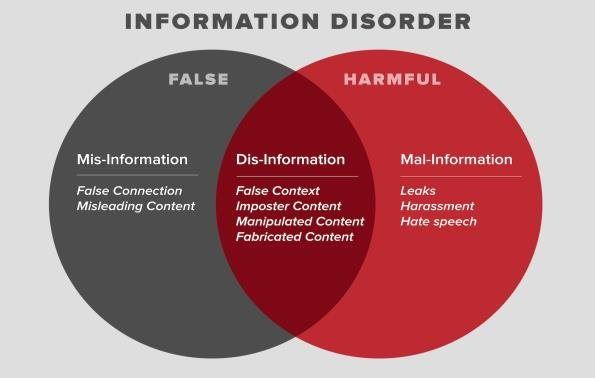
\includegraphics[width=\linewidth]{figures/fig_disorder.jpg}
    \caption{真実性・有害性による情報の分類と概要例\cite{wardle2017information}.}
    \label{fig:info}
\end{figure}

% \section{偽情報の詳細な分類}
% 一口に悪意によって意図的に作られた事実に反する情報と呼んでも,情報作成者の意図に悪意がどれだけ入ってくるかによって危険性は変わる.
% 偽情報が含まれるMis-informationとDis-informationは読者を欺こうとする悪意の度合いによって7種類に分けられるとしている\cite{wardle_2017}.
% 図\ref{fig:types}は左から右の順に以下を説明している.

% \begin{itemize}
%     \item \textbf{Satire or parody}: 皮肉あるいはパロディ.危害を加える意図はないが,読者を騙す可能性をもつ.最も悪意が少ない.
%     \item \textbf{False connection}: 見出しやキャプションが内容と乖離している.
%     \item \textbf{Misleading content}: ミスリード.情報を誤解を招く方向に利用している.
%     \item \textbf{False context}: 本当の内容が虚偽の文脈情報で共有されている.
%     \item \textbf{Imposter content}: 情報源として虚偽のものを使っている.
%     \item \textbf{Manipulated content}: 本当の情報や画像を操作して騙そうとしている.
%     \item \textbf{Fabricated content}: 新しい内容が完全に虚偽であり,騙して実害を与えようとしている.最も悪意が多い.
% \end{itemize}

% \begin{figure}[p]
%     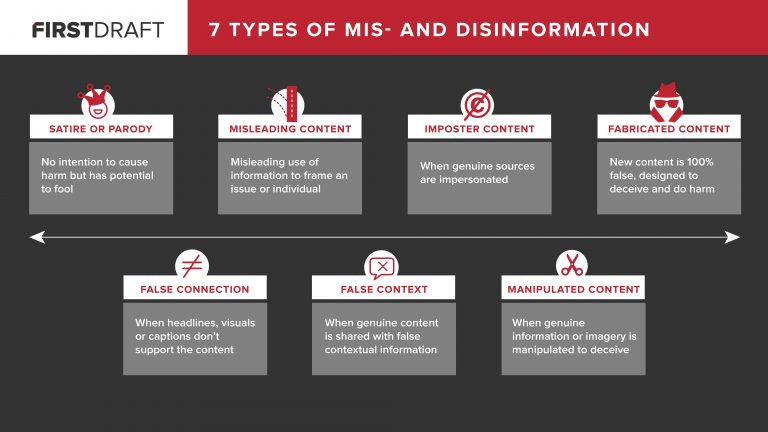
\includegraphics[width=\linewidth]{figures/fig_types.jpg}
%     \caption{誤情報(Mis-information, Dis-information)を作者の悪意の程度によって7種類に分類した図\cite{wardle_2017}.}
%     \label{fig:types}
% \end{figure}


\section{偽情報がもつ危険性}
近年でも、\cref{ch:introduction}で示した2022年のロシアによるウクライナ侵攻に関連した偽情報 \cite{evon_2022}に限らず、
2023年のパレスチナとイスラエルの戦争、そして2024年の能登半島地震といった社会情勢の変化に便乗した偽情報が投稿されている \cite{Press_2023,noto}。
これらの偽情報が拡散されることで発生する問題点は多岐にわたる。

\subsection{世論の操作}
偽情報の影響により世論が誘導された可能性がいくつか指摘されている.

例えば英インデペンデント紙は英国のEU離脱国民投票において,
図\ref{fig:leave}のように
「EUを離脱して毎週の拠出金3.5億ポンドをNHS(国民保険サービス)に供給しよう」といった主張\cite{merrick_2018}をはじめとする偽情報が選挙期間中に流布された結果,
離脱派の勝利に繋がった可能性が指摘されている\cite{grice_2017}.

また米ニューズウィーク誌によると2016年大統領選挙では,SNSプラットフォームで偽情報を含む情報によるターゲット広告を閉鎖的なコミュニティの中で発信することで,
有権者の支持を得ることに成功したと指摘している\cite{burleigh_2017}.

\begin{figure}[p]
    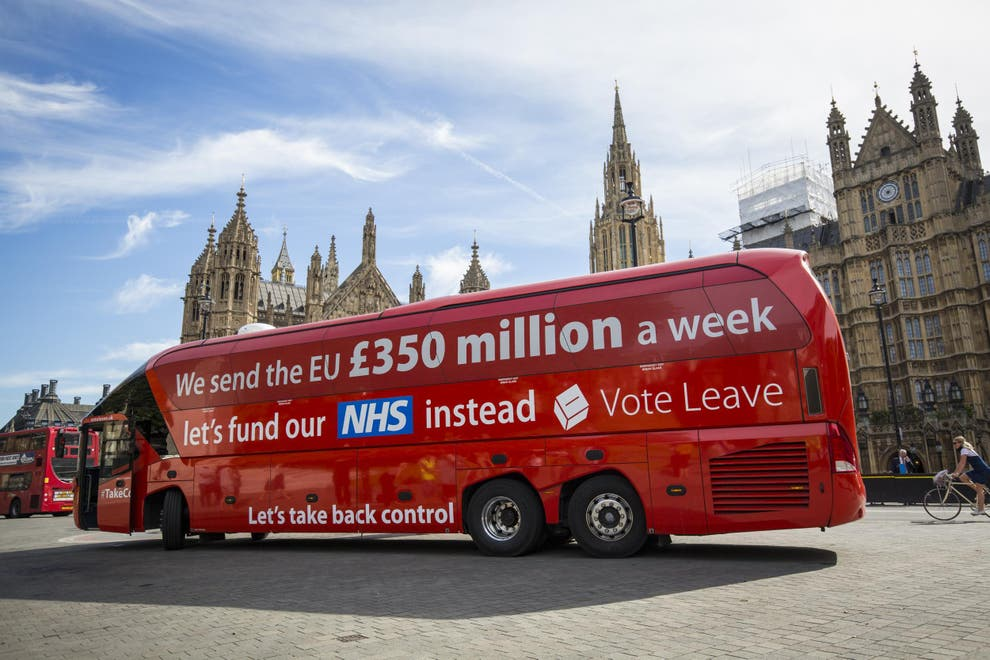
\includegraphics[width=\linewidth]{figures/fig_leave.jpg}
    \caption{英国でEU離脱の是非を問う国民投票の事前運動で出された広告.「EUを離脱すれば毎週払っている3.5億ポンドの拠出金をNHS(国民保険サービス)に供給できる」としているが,後にこれが誤りだった可能性を認めている\cite{merrick_2018}.}
    \label{fig:leave}
\end{figure}

このように、偽情報によって国民が正しい情報にアクセスできない場合、世論が操作され選挙結果にも影響を与えうる。
これを象徴するように、2024年の世界経済フォーラム年次総会(通称、ダボス会議)に先立って公開されたグローバルリスク報告書2024年版にて、今後2年間において最も重要・深刻なグローバルリスクとして「誤報と偽情報」(``Misinformation and disinformation'')を挙げたうえ、
今後10年間における重要さでも誤報と偽情報は全体の5位であるほか、学術領域から最も多く挙げられたグローバルリスクも誤報と偽情報と報告されている \cite{wef2024,wef2024_j}。
主な理由として、今後数年間に米国やインドといった超大国で選挙が予定されている点が挙げられている。

\subsection{事件への影響}
また実際に発生した事件に偽情報が影響を及ぼした事例も数多く報告されている.

例えば2016年米国大統領選挙期間中に「ワシントンDCの民主党支持者が経営するピザ屋は小児性愛者と児童売春の拠点となっており,ヒラリー・クリントン候補(当時)が関与している」という
偽情報が流布された結果,それを信じた者により銃撃事件に発展した \cite{agencies_2016}.
同じように偽情報が陰謀論の信奉者を増やした例としてQアノンが挙げられる.
これは「政財界とマスコミにエリートとして巣食う悪魔崇拝の小児性加害者たちに対して、トランプ前大統領は秘密の戦争を繰り広げている」という旨の内容である \cite{wendling_2021}が,
2021年1月に発生した米国議会襲撃事件にて,多くの信奉者が逮捕された \cite{hymes_mcdonald_watson_2021}.
このような陰謀論を人々に信じ込ませる手段として偽情報がSNSの発信を介して利用されている状況について,
WWW(ワールド・ワイド・ウェブ)を発明したティム・バーナーズ・リーは不快感を示すとともに対策を呼びかけている \cite{reklaitis_2018}.

これに加え偽情報によって株価が影響を受けたケースもある.
2013年にAP通信のTwitterアカウントが乗っ取り被害を受け,
「ホワイトハウスで爆発がありオバマ大統領(当時)が怪我を負った」というツイートが発信された影響で,
一時株式市場から約1360億ドルが消失した \cite{fisher_2013}.
またインドではテキストチャットアプリのWhatsAppで暴力を扇動する情報が拡散された影響で,
多くの集団暴行致死事件が発生したと報告されている \cite{frayer_2018}.

2024年夏では、イングランドで反移民や反イスラムを主張する極右支持者らによる暴動が各地で発生した。
この発端は、サウスポートで発生した殺人事件の犯人の出自に関する偽情報がソーシャルメディア上で拡散されたためであった \cite{Spring_2024}。

\subsection{公衆衛生への影響: 新型コロナウイルス感染症(COVID-19)}
新型コロナウイルス感染症の流行により,SNS上では真偽が疑わしい感染症に関する情報が多く流布された.
これまで流行した新型感染症であるSARS(重症急性呼吸器症候群)やMERS(中東呼吸器症候群),
そしてジカ熱との違いとして,SNS上で恐怖を扇動する動きが見られた点が指摘されている.
WHOはTwitter・Facebook(当時)・Tencent(中国のテキストチャットアプリWeChatを運営する)・TikTokと連携し,
偽情報を取り締まることで抑え込みを図っている\cite{hao_2020}.

また2015年から言語・事例を問わずEU加盟国・近隣諸国に関する偽情報を集積するEUvsDisinfoプロジェクト\cite{euvsdisinfo_2020}は,
8000件を超える事例のうち直近1000件の大半が新型コロナウイルス感染症に関連する記事を含んでいる\cite{euvsdisinfo_2020_2}など,
このトピックに関連する偽情報対策を目的とした取り組みが行われている.

\section{偽情報を話す偽音声の出現}
近年の新たな傾向として、偽情報の媒体が多様化している点が挙げられる。
これまで偽情報は記事文章と写真が中心であったが、ソーシャルメディアが扱う媒体が多様化するにつれ拡散される偽情報も文章や画像以外の形式が増えている。
具体的な事例として映像と音声による偽情報を\cref{ch:introduction}にて紹介したが、媒体によって偽情報の拡散の傾向に違いがあるのか研究した論文がある。
Davidsonと小林の論文 \cite{DAVIDSON2022107241}によると、前述の米国議会襲撃事件に影響を与えたとされる偽情報の拡散傾向を分析した結果、
画像による偽情報に比べて映像による偽情報の方が多く拡散されたと報告している。

また、音声合成手法によって虚偽の主張を行い送金を要求する詐欺行為も複数件発生している。
2019年に架空企業のCEOになりすまして振り込みを行うよう電話で指示する事案が発生した \cite{Stupp_2019}ほか、
2023年には実在企業の役員に事前に許可を得てなりすまして、部下の従業員から金銭を得ることに成功したと報告されている \cite{Bunn_2023}。
成功した要因として本人の電話番号を乗っ取った上でテキストチャットを送った点も挙げられているが、YouTubeから得た十数分程度の音声サンプルをAIに学習させて取得したなりすまし偽音声を送った点も挙げられている。


\section{ファクトチェック}
対象となるニュースがもつ情報が真実かどうか有識者が行うファクトチェックが偽情報対策として行われている.
英語圏ではファクトチェックプラットフォームとしてPolitiFact(政治ニュース専門)とGossipCop(芸能ニュース専門)の他にもFACTCHECK.ORGやSnopes,Full Factなどが活動している.
また日本国内では日本ファクトチェックセンターが活動しているほか、認定NPO法人であるファクトチェック・イニシアティブがファクトチェックの推進活動を行っている。
現在全世界で活動しているファクトチェック団体は2020年10月に300ヶ所を超え,前年に比べ約100ヶ所増加したと報告されており,
特にアジア圏では2016年に比べ活動団体数が3倍以上に増えたという\cite{stencel_luther_2020}.

これらのファクトチェックに関与する団体が加盟する国際ファクトチェックネットワーク(International Fact-Checking Network, IFCN)では,
``Code of Principals''としてファクトチェックを行う際の5原則が示されている\cite{IFCN,fij}.

\begin{itemize}
    \item \textbf{A commitment to Nonpartisanship and Fairness}: 非党派性と公正性.すべてのファクトチェックを同じ基準で行い,ファクトチェックする問題について一切の唱道や政治的立場をとってはならない.
    \item \textbf{A commitment to Transparency of Sources}: 情報源の透明性.読者自ら調査結果へ至った経緯を確認できるようにする.情報源の個人的安全の保護を除き,詳細な情報を提供すること.
    \item \textbf{A commitment to Transparency of Funding \& Organization}: 財源と組織の透明性.外部から資金提供を受けたとしても,提供者がファクトチェックに影響を及ぼしてはならない.また組織における全重要人物の職業的背景や連絡先を明記し,組織構造と法的地位を公開すること.
    \item \textbf{A commitment to Transparency of methodology}: 方法論の透明性.ファクトチェックの選択、調査、執筆、編集、公表、修正に使用している方法を説明し,ファクトチェックする理由と方法を示すこと.
    \item \textbf{A commitment to Open \& Honest Corrections Policy}: 明確で誠実な訂正方針.訂正方針を公表し,厳格に運用する.その方針に則り,読者に訂正記事を明確かつ透明性をもって表示されるように務めること.
\end{itemize}

IFCNに加盟を希望するファクトチェック団体は,これらの原則を遵守しているか審査を受けて認可を受けることで加盟となる.
加盟後も原則を遵守しているか定期的に審査が行われており、2024年現在審査を通過した団体が122あり、そのうち4団体が日本国内で活動を行っている \cite{IFCNCoP}。



\section{ファクトチェックの問題点と早期発見の重要性}
\subsection{検証が属人的}
ファクトチェックは手続きの内容上,特定のカテゴリやドメインに対する深い知識や発信者や関係者との関係を必要とする.
組織によってファクトチェックを行う専門職が用意されている場合があり,
近い職業として編集者・校正者・記者が挙げられている\cite{deahl_2019}.

一方でソーシャルメディア利用者によるファクトチェックとして、一部プラットフォームが投稿に補足情報(コミュニティーノート)を追記する機能で部分的に実装が行われている。
このようなクラウドソーシングによる事実確認は、部分的には専門家の結果に近い傾向を示す一方で、バイアスが強くかかった一部の集団による影響を受けやすいと指摘されている \cite{10.1145/3511808.3557279}。

\subsection{結果発表に時間がかかる}
ファクトチェックでは,場合によっては記事にて情報源としている相手とのやり取りなどを行う必要があるため,
真偽がわからないまま時間が経過する.
\cref{ch:introduction}で記述したように、\cref{fig:example}では偽情報投稿からファクトチェック結果まで25日間かかっていた.
もし発信から偽情報と突き止めるまで時間がかかると,その間は偽情報がSNSで拡散され続けることを意味する.
また時間が経ったことにより,利用者へ該当情報が虚偽である点が伝わりにくくなり,拡散されずに更に利用者へ結果が周知されなくなる可能性がある.

利用者によるファクトチェック結果として偽情報の疑いが強いとする補足情報が付与された場合でも、
付与前後に当該情報の表示傾向に変化が見られない上に、
そも補足情報の付与が拡散の初期段階に間に合っていないと指摘されている \cite{chuai2023rollout}。

現に、ファクトチェックによって既に偽情報と確認されている多くの情報が、
未だに利用者によって事実と認識されているという報告もある \cite{真一_2023}。
よって,自動に早期検出して利用者へ注意喚起することが求められている.

\cleardoublepage
\chapter{関連研究}\label{ch:rel_res}

偽情報および偽情報の自動検出(真偽分類)は,対象にスパム\cite{shen2017discovering}や風評\cite{7023340},そして虚偽広告\cite{Huang:2017:DFO:3041021.3054233}を含めると新しいトピックではない.
\cref{ch:introduction}の通り,本研究はこれまでの研究\cite{Born2017-11-02,Shu:2017:FND:3137597.3137600,Ruchansky:2017:CHD:3132847.3132877,Wang:2018:EEA:3219819.3219903}に倣い,人を混乱させ惑わすために意図的・意識的に作られたウソ、虚偽の情報を偽情報と定義する.
なお、関連する単語として誤情報(誤報、misinformation)もあるが、これは勘違いや誤解により拡散された間違った情報を指すものとして区別されている\cite{Born2017-11-02,gov2024}。

本章では、偽情報の自動検出を行う研究で事実確認を行うファクトチェックの補助と情報生成技術の発展、偽情報の自動検出を通して既存研究が抱える問題点を指摘する。


\section{ファクトチェックの補助}
ファクトチェックを補助することが目的である研究は数多く,実現する方法によっていくつかに分けられる.

\subsection{ファクトチェックを必要とする言説の自動検出}
事実かどうか疑わしく,ファクトチェックを必要とする言説がどこにあるか自動で評価する研究が行われている.
例えば,ClaimBusterは米国大統領選挙のテレビ討論会で候補者が話した内容からファクトチェックを必要とする重要な言説を自動で検出するものである\cite{10.1145/2806416.2806652}.
これを発展させ,マルチタスク学習によって精度を向上させたモデル\cite{vasileva-etal-2019-takes}が提案されているほか,
インタビューやニュース記事,そして英語に加えアラビア語に対応したClaimRank\cite{jaradat-etal-2018-claimrank}が提案されている.
毎年開催されているCheckThat!では,演説やニュース記事からファクトチェックが必要な部分を検出する共有タスクが提供されている\cite{10.1007/978-3-030-45442-5_65}.
例えば2024年開催では、共有タスクの1つとして英語・オランダ語・アラビア語の投稿での手法の公募が行われ \cite{hasanain2024overview}、
参加手法では多くの大規模言語モデルを活用した手法が提案されている \cite{gruman2024clac,golik2024dshacker,li2024factfinderscheckthat2024refining,roysland2024iai,aguilera2024sinai,bulut2024turquaz}。

また日本国内では,事実かどうか疑わしくファクトチェックが必要なTwitterのツイートを自動で検出するモデルも提案されている\cite{内山香2018}.

\subsection{ファクトチェックの自動化}
ファクトチェックの自動化はいくつかの方面からアプローチがとられている.

例えば言説から既にファクトチェック済である部分を自動で検出するモデル\cite{shaar-etal-2020-known}が提案されている.
他にはFEVERというWikipedia上の記述を解析し事実に基づくかどうか判断するモデルも提案され\cite{thorne-etal-2018-fever},
改善モデルとしてグラフネットワークを採用されたモデル\cite{zhong-etal-2020-reasoning}や,共有タスクにより性能に改善がみられたと報告されている\cite{thorne-etal-2019-fever2}.

表やデータベースを利用した自動ファクトチェックの研究も幾つか行われている.
Wikipedia上の表データに基づく言説とそうではない言説を集めたデータセットが提供されており\cite{chen2020tabfact},
他にも入力された言説文章からデータベースでSQLを自動で発行し情報を確認するStructinizer\cite{10.14778/3407790.3407841}も提案されている.

構造化データベースの一種であるナレッジグラフを利用して事実確認を容易に行えるようにするツールも提供されている.
Tracyモデルは与えられた背景知識から、文章とナレッジグラフをもとに確認したい事実を平易な内容に書き下すツールを提供するものである\cite{10.1145/3308558.3314126}.

また偽情報はそうでないニュースと比べて内容が複雑であることに着目し,事前に用意した証拠情報と類似度が高い言説との関連度(パープレキシティ)を算出し,そのスコアで真偽を判断するモデルが提供されている\cite{lee2020misinformation}.

公衆衛生など専門知識を要する分野での検証結果に信憑性を持たせるために、説明を伴った検証結果を生成する手法\cite{kotonya-toni-2020-explainable-automated}や、質問応答形式による説明可能性の導入\cite{9747214}も提案されている。


\section{情報の生成}
本節では、偽情報を取り巻く状況に大きな影響を与えた情報の生成技術の発展について記述する。

\subsection{大規模言語モデルによる自然言語文章生成}
自然言語処理における文章生成タスクは、古くは1950年代から既に統計的ないしは構造化された手法\cite{Fine1998,10.1162/089120102762671972}が提案されていた。
一方で、自然言語は機械言語と違い表現に柔軟性と独創性があるため自然な文章の生成には難点があった。
近年では,深層学習をベースにした言語モデルの発展によりその課題が改善されつつある.
特にEncoder-DecoderからなるAttention機構を取り入れたTransformerモデルの提案\cite{NIPS2017_3f5ee243}が大きな現状打破を生み出した.
この派生型として,TransformerのDecoderを利用し文章生成に特化したGenerative Pre-trained Transformer 2(GPT-2)が提案\cite{Radford_GPT2}されており,
開発側はその性能からモデル公開に対して偽情報生成をはじめとする悪用に対した懸念を表明している\cite{solaiman_clark_brundage_2020}.
この他にもTransformerのEncoderを利用したBERT\cite{devlin2019bert}以降、より自然な文章を生成できるモデルが多数提案されている.

この頃からパラメータの規模を大きくした言語モデルは大規模言語モデル(Large Language Model, LLM)と呼ばれており、特に2022年以降に注目を集めている。 %TODO: 論文統計
中でもGPT-2のパラメータ数15億から1750億まで増やしたGPT-3では,テキスト生成タスクにおいて人間が作成した文章と遜色ないクオリティを提供できたと報告されている\cite{brown2020language}.
このモデルが提案された当初では数学課題や学習データによる倫理的バイアスに対して課題が指摘されていた\cite{Floridi2020,Chan2023}ものの、
モデルの調整\cite{borchers-etal-2022-looking}や指示方法の最適化\cite{NEURIPS2022_8bb0d291,NEURIPS2022_9d560961}によって改善がみられている\cite{DBLP:conf/aied/AnLG23}。
またGPT-3をベースに、対話応答タスクに対する利用者側のフィードバックを基準にした強化学習を行うInstructGPTも提案されており\cite{NEURIPS2022_b1efde53}、
ベースモデルのパラメータ数を拡張させたGPT3.5を使用した対話応答AIはChatGPTとして一般に提供されている\cite{RAY2023121}。
また、更にパラメータ数を拡張させたGPT-4も提案され、質問応答に限らず広範なタスクの成績が改善されている\cite{openai2023gpt4}。
GPTを開発するOpenAI以外では、GoogleによるGemini \cite{geminiteam2024geminifamilyhighlycapable, geminiteam2024gemini15unlockingmultimodal}のほか、
公開された言語モデルとしてMetaによるLLaMA \cite{touvron2023llamaopenefficientfoundation}はその後 Llama 2 \cite{touvron2023llama2openfoundation} 及びLlama 3 \cite{dubey2024llama3herdmodels} が提案されている。


\subsection{偽情報記事生成}
\label{sec:generate}
このような自然言語文章生成技術の発展と同時に、偽情報を含めた架空の情報の生成を行うモデルも提案されている。
自然言語生成モデルの1つとして,架空のニュース記事を作成するGroverモデルがある\cite{DBLP:journals/corr/abs-1905-12616}.
このモデルはニュース記事データセットから記事をドメイン・著者・投稿日時・見出し・本文の5要素に分け,無作為に要素を削除した記事の残り部分から歯抜け部分を予測させることで訓練している.
興味深い点として,Groverモデルで生成した記事の方が実在の記事よりも読者が信じやすい傾向が報告されていた.

この偽情報生成によって人間を実際に欺くことができるのか,別の研究で本文と画像とキャプションをセットにした架空の記事と実在の記事を読者に見せる実験が行われた.
その結果,視覚的・意味的矛盾が発生しなければ利用者は騙される可能性が指摘されている\cite{tan-etal-2020-detecting}.

\subsection{音声生成}
音声合成技術も深層学習の影響で急激な進歩を遂げている。
特にTTSは2019年頃まで事前学習によって音響 \cite{6639215,8461368}や言語特徴 \cite{vandenoord16_ssw}を学習してから、
別モデルが音声波形を生成させる機能を学習する形をとっていた \cite{vandenoord16_ssw,pmlr-v80-kalchbrenner18a}。
この場合だと学習の段階が複雑化しやすいため、学習から生成まで単一のモデルで一貫した生成学習プロセスを目指した研究もある \cite{wang17n_interspeech,ren2021fastspeech,donahue2021endtoend}。
また変分オートエンコーダーを利用した手法も提案されており、より人間らしい自然な声が得やすくなっている \cite{pmlr-v139-kim21f,https://doi.org/10.48550/arxiv.2205.04421}。
この急速な進歩の影響により、
2019年以前の音声合成手法をベースにした合成音声検出手法は、
新たに2021年にまでに提案された音声合成手法による音声を検出できなかったという報告が
寄せられている \cite{yamagishi21_asvspoof,yu_icmece}。

\section{偽情報の自動検出}
\subsection{記事内容を入力とする偽情報検出}
TwitterのようなSNSを対象とした情報の信憑性を自動評価する研究は2011年に既に投稿内容や投稿者,そして拡散経緯を使用する手法が提案されている\cite{10.1145/1963405.1963500}.
また時間経過によって風説に関する情報の増加による言説の変化に再帰型ニューラルネットワーク(RNN)で対応したものが提案されている\cite{10.5555/3061053.3061153}ほか,
SNS上の噂の信憑性を推定する共有タスクが2017年に提供され\cite{derczynski-etal-2017-semeval},発展型として噂をつぶやくツイート群にそれぞれ寄せられた議論のツイートも対象に含んだ共有タスクも提供されている\cite{gorrell-etal-2019-semeval}.

またニュース記事がもつ情報から偽情報を検出する手法は多く提案されている.
文字情報からは,偽情報が独自の書かれ方をする上に感情的な表現を多用することから,文章のスタイル\cite{potthast-etal-2018-stylometric}や感情的表現の頻度\cite{DBLP:journals/corr/abs-1903-01728}を考慮する手法がある.
また,ディープニューラルネットワーク(DNN)によって検出性能が改善された報告\cite{wang-2017-liar,karimi-tang-2019-learning,karimi-etal-2018-multi}も多い.
特に検出においてもTransformerを利用した手法は多く、BERTを利用した手法で性能が改善した報告がある \cite{Kaliyar2021,yanagi2021classifying}。
他にもGPT-3.5に対して偽情報記事の例を示すことによって、学習データを増やす手法も提案されている \cite{lucas-etal-2023-fighting}。
Beizhe Huらによる研究 \cite{Hu_Sheng_Cao_Shi_Li_Wang_Qi_2024}では、大規模言語モデルのGPT3.5-turboを一部組み込んだ手法を提案している。
またLingyao Liらによる研究 \cite{10.1145/3643829}では、Hate/Offensive/Toxicの3観点に該当する投稿をChatGPTに検出させた結果、いずれのラベルに該当する場合のF1-scoreは0.39~0.67と報告している。
他の報告によると、単純にLLMに対して情報を入力するだけでは性能が悪いため、LLMが情報の背景を理解しやすいように入力情報を調整した場合性能が改善した \cite{doi:10.1137/1.9781611978032.50}。
LLMに限らず、入力記事に加えて詳細を解説する記述を追加することは比較的簡易的な機械学習手法の検出性能を改善できるという報告もある \cite{Bonet-Jover2024}。

\subsection{利用者の反応を活用した偽情報検出}
コメントやRP(リポスト、RT/リツイートとも)といった記事に対する反応であるソーシャルコンテキストを考慮した手法も多く提案されており,扱うコンテキストの種類によってユーザベース\cite{Castillo:2011:ICT:1963405.1963500,8397048,DBLP:journals/corr/abs-1904-13355}
・投稿ベース\cite{Yang_Shu_Wang_Gu_Wu_Liu_2019,Tacchini2017SomeLI,Jin:2016:NVE:3016100.3016318}
・ネットワークベース\cite{Wu:2018:TFF:3159652.3159677,DBLP:journals/corr/abs-1902-06673}の3種類に分けられる.
また,投稿と反応を寄せたユーザ情報と併せて検出を目指した研究も報告されている\cite{10.1145/3386253}.

記事内容と記事に対して寄せられたコメントを併せて検出を行う手法も幾つか提案されており、双方向リカレントニューラルネットワーク(RNN)を導入した手法や\cite{https://doi.org/10.1049/ise2.12021}、
コメントが指摘している部分を記事中から可視化する手法 \cite{10.1145/3292500.3330935}、
各コメントの姿勢(賛同/中立/否定)を自動で判定する形で判定を補助する手法 \cite{9414787} などが提案されている。
また、生成AIによるコメント生成を活用した早期検出の実現へ,TCNN-URGという2層の畳み込みニューラルネットワークと条件付き変分オートエンコーダ(CVAE)によるユーザレスポンス生成器を組み合わせたモデルも提案されている\cite{ijcai2018-533}.
また、動画に対してユーザのコメントも含めた総合的な観点から偽情報検出を行うモデルも提案されている \cite{zong-etal-2024-unveiling}。

\subsection{音声を対象とした偽情報検出}
偽情報が発信される形式の多様化によって、架空の主張を行う偽音声の危険性が強まっている。
\cref{ch:introduction}の通り、偽音声の検出はもともと生体認証システムに対するなりすまし攻撃を想定した対策が研究されていた。
なりすまし音声による攻撃としてASVspoofは2021年以前の段階では、合成音声を電話回線を介して入力される場合と録音再生された場合の2種類を想定したシナリオを用意した \cite{7858696}。
使用される合成音声の形は、文章を入力に使うText-To-Speech(TTS)と、
話者音声を別人の音声へ変換するVoice Conversion(VC)の2種類である。
2021年の開催では、新たに合成音声をオンラインを介して公開された場合を想定したシナリオが追加された \cite{yamagishi21_asvspoof}。
このシナリオには本研究が目的とするSNS上で投稿された場合も含まれる。
ASVSpoofは隔年で開催されており、
2021年開催のデータセットでは2019年までに提案されている手法で学習を行った。
またこの大会に参加しなかった研究でも深層学習を利用して良好な検出性能を得た報告もある \cite{10.1145/3394171.3413716}。

\section{音声分析形式の種類}
音声を入力とする話者認識(Speaker Recognition)には、話者識別(Speaker Identification)と話者照合(Speaker Verification)という2種類の形式がある \cite{FURUI1997859,628714,5745552}。
\cref{fig:speaker_recog}は2種類の形式の違いを示す。

\begin{figure}[p]
    \centering
    \begin{minipage}{0.9\linewidth}
        \centering
        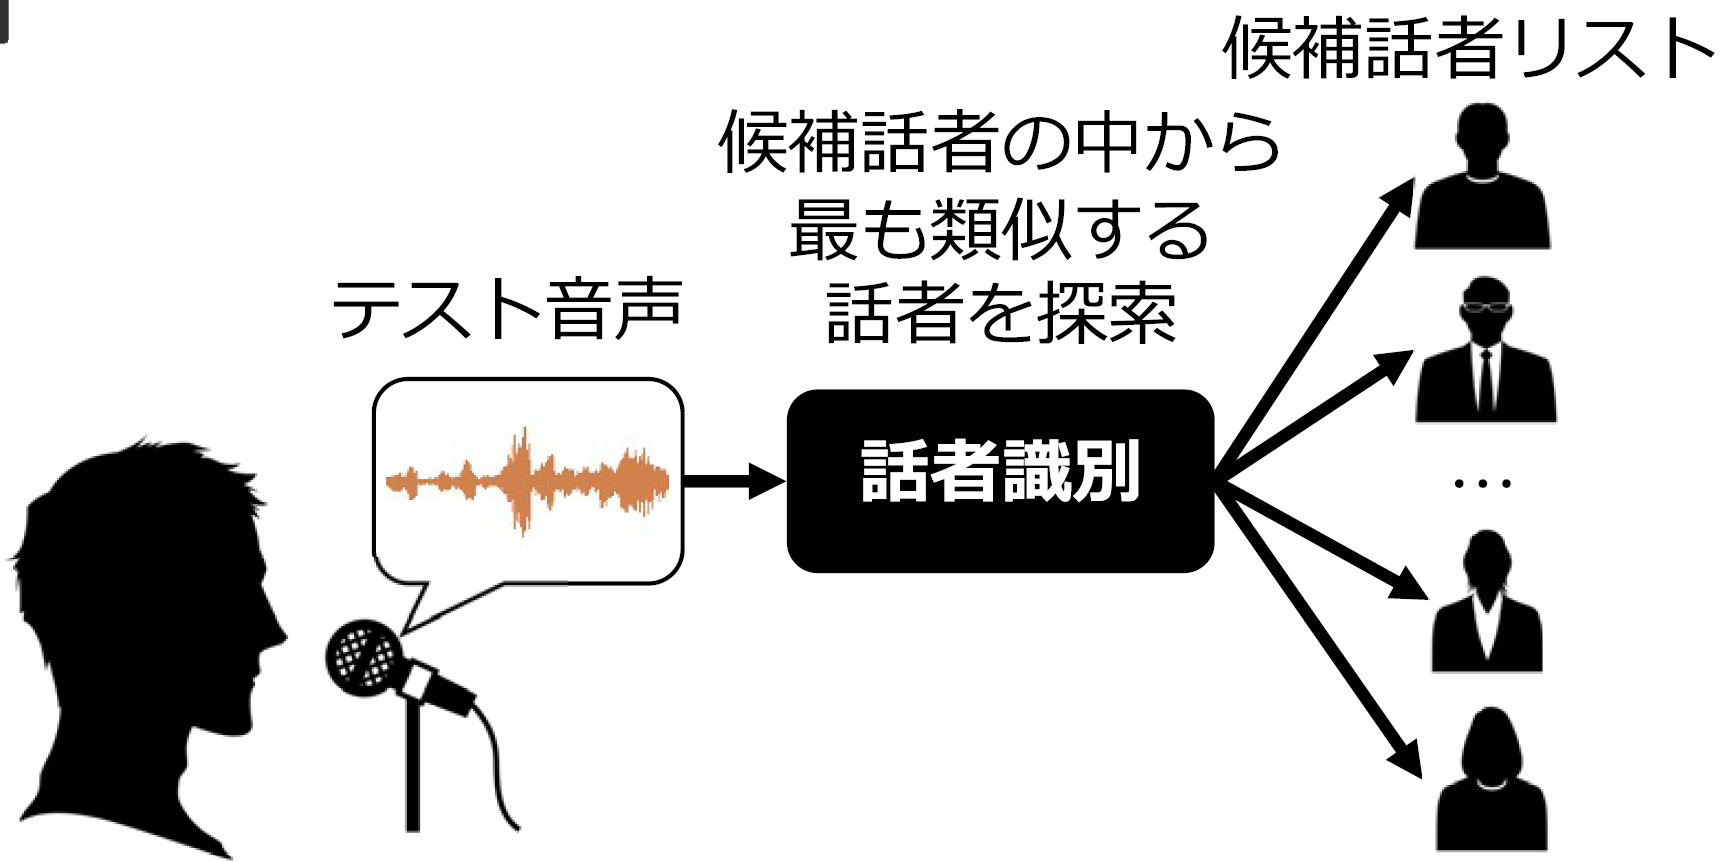
\includegraphics[width=0.8\linewidth]{figures/sd.png}
        \subcaption{話者識別}
    \end{minipage}
    \begin{minipage}{0.9\linewidth}
        \centering
        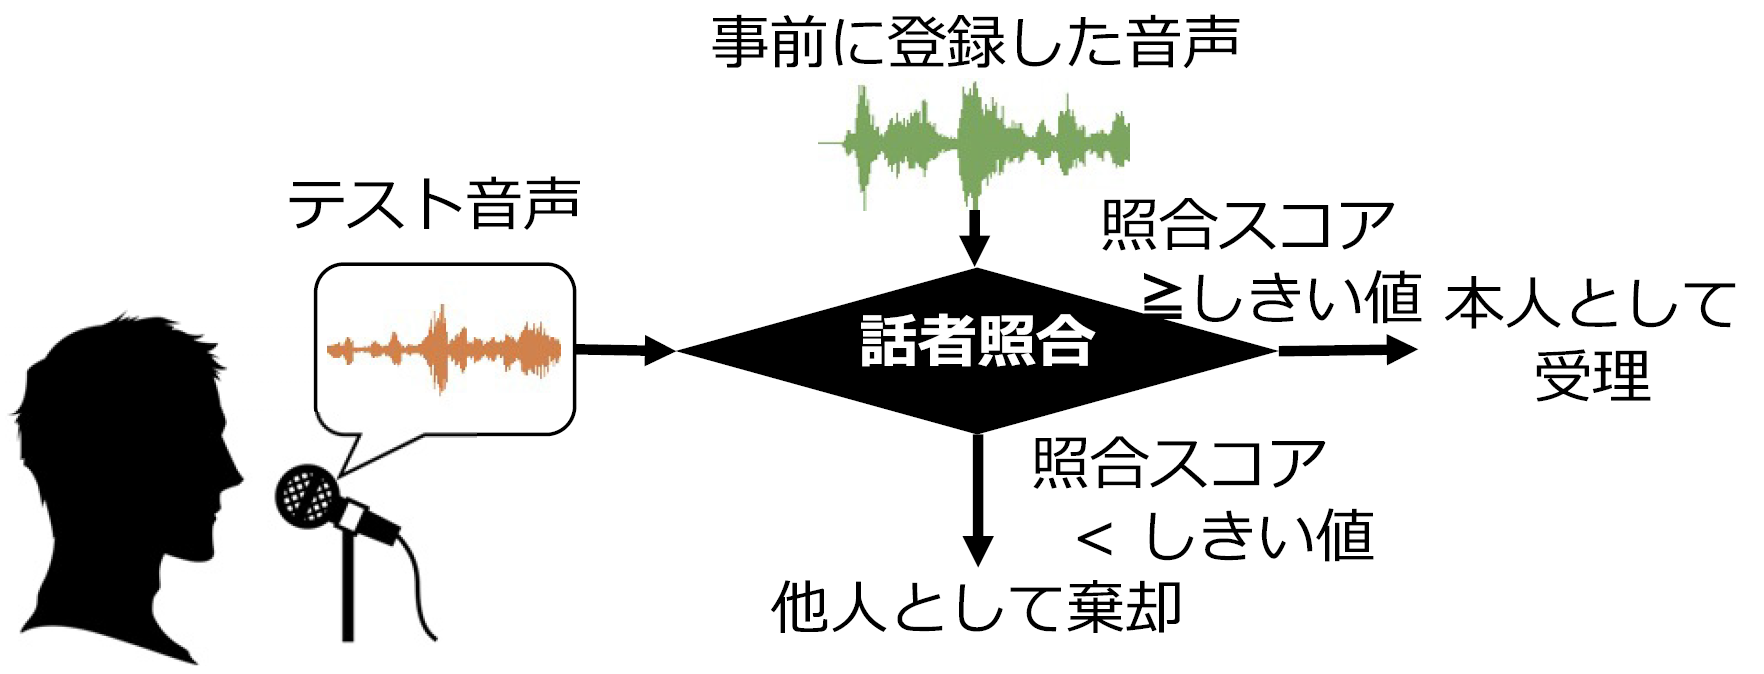
\includegraphics[width=0.8\linewidth]{figures/sv.png}
        \subcaption{話者照合}
    \end{minipage}
    \caption{話者認識の形式 \cite{俵直弘2022}}
    \label{fig:speaker_recog}
\end{figure}

話者識別は事前に登録した複数の候補者の中から提示された音声の話者を探索する1対nの推定問題であるのに対し、
話者照合では,提示された二つの音声が同一話者によるものか否かを推定する1対1の照合問題として定義する \cite{俵直弘2022}。
識別では、未知の話者を既知の話者のデータベースと比較し、最もよく一致する話者を識別結果として与える。
一方で照合では、音声サンプルが主張された人物によって話されたかどうかを判断するタスクと言える \cite{1561284}。
よって、本研究で行うなりすまし偽音声の検出は、話者照合に該当する。

また,話者認識は,登録時と照合時で同じ内容の音声を用いるテキスト依存型(text-dependent)と,
登録時と照合時で異なる内容の音声を用いるテキスト独立型(text-independent)に分類される \cite{俵直弘2022}。
% ASVspoofにおけるなりすまし検出では、テキスト依存型の形式を取っている。
% 読み上げる音声は本人・偽いずれも新聞記事から引用した同一の文章を読み上げているため、
% 実際にSNS上で偽音声による偽情報が投稿された状況から乖離がある。
% よって本研究では、テキスト独立型の話者照合を行う。

\section{既存手法の問題点}
\subsection{コメントと早期検出の相性}
コメントを含めたソーシャルコンテキストを利用する手法に共通した問題点として,ソーシャルコンテキストはユーザの拡散によって生まれる情報であるため早期検出に向かない点が挙げられる.
先述のCVAEによるユーザレスポンス生成器を組み合わせたモデル\cite{ijcai2018-533}では、
ニュース記事を畳み込みニューラルネットワークで特徴化してから隠れ変数を算出し,寄せられたコメントとして尤もらしい単語群を生成することで検出性能が改善されることが報告されている.
しかしながら,TCNN-URGはあくまで尤もらしい単語を生成することに限られ,実際のコメントそのものは生成していない.

また、コメントを考慮するモデルに対して誤った判断へ誘導するコメントを生成する手法も提案されており \cite{9338282}、これは外部から与えられる情報のみに依存する危険性を示している。

\subsection{偽情報形式の多様化}
近年では、偽情報がもつ形式が文章に限らず多岐にわたる傾向にある。
記事と画像を併せて発信された情報に対する自動検出手法 \cite{10.1145/3219819.3219903,8919302}はすでに幾つか提案されているものの、
動画や音声など生成技術の発展により対応が必要な形式の領域が急速に広がっている。

特に既存の偽音声検出手法の多くは、新聞記事を読み上げた人間の音声と合成音声を使ったデータセット \cite{wu15e_interspeech,WANG2020101114}を検出対象としている。
その影響で基本的に音声波形そのものを手法の入力として扱っており、
対象音声がどのような内容の主張を行っているかは考慮に入れていない。

\subsection{検出性能の維持}
偽情報の検出は、偽情報生成側とのいたちごっこが続いている。
元々ニュース記事を検出する場合でも、ドメイン(分野)固有の要因による検出性能の維持の難しさによって、新規ニュースに対して性能維持が難しい点が指摘されている \cite{10.1145/3459637.3482139}ほか、
同一のニューストピックを扱う別々のデータセット間でも、検出性能に大幅な差が出る点もまた指摘されている \cite{10.1007/978-3-030-73696-5_13}。

さらに、GPT-4を始めとするLLMの影響によって偽情報文章の生成が誰でも容易になった点も指摘されている \cite{DWIVEDI2023102642}。
この影響により、今後出現する偽情報はこれまで以上に既存の検出手法を掻い潜りやすくなる点が見込まれる。


\cleardoublepage
\chapter{コメント生成による検出補助}\label{ch:gen_com}
\section{目的}\label{sec:gen_pur}
\label{ch:purpose}
\subsection{対象}
今回対象とする情報は,既にファクトチェックによって真偽が評価されているニュースと,ニュースに対してSNS上で寄せられたコメントである.
データセットの詳細な仕様は\cref{sec:dataset}で説明する.
真偽はデータセットが採用しているReal・Fakeの2種類である.
また今回対象とする言語は英語である.

実際に実験で使用したReal・Fakeの例が表\ref{tbl:data_example}の通りである.いずれも芸能記事を専門とするファクトチェックプラットフォームであるGossipCopにファクトチェックされ真偽が公表されているものである.
Realの例は俳優のエディ・シブリアンが,女優のリアン・ライムスによる「不健康な行動」に関する告発へ反論する記事\cite{calvario_2017}とコメントを示している.
一方Fakeの例は英国キャサリン妃とメーガン妃は永遠の親友と言えるほど完全に良好な関係ではないかもしれないとする記事\cite{bahou_2018}とコメントを示している.

表\ref{tbl:data_example}のコメントによると,Realのコメントは記事のタイトルを記述した投稿が中心であるが,
Fakeのコメントは特に3件目のように信憑性に疑問を投げかけている.
このことから,コメントを考慮することで,ユーザによる反応から真偽を判断するにあたって有力な手がかりを得られることが予想される.
ただし早期検出に向けて検出実験で使用できるコメントの数が制限されるため,必ずしもそういった情報が得られる訳ではない点に留意が必要である.
\begin{landscape}
\begin{table}[h]
    \centering
    \caption{実験で使用した記事本文の冒頭と実在コメント3件の例.いずれもGossipCopでファクトチェックされている.}
    \label{tbl:data_example}
    \begin{tabularx}{\linewidth}{llX}  \hline
        ラベル & 項目 & 内容 \\ \hline
        \multirow{4}{*}{Real} & 記事                         & \texttt{The drama between Eddie Cibrian and Brandi Glanville continues.  The 43-year-old actor fired back at his ex-wife after she accused Cibrian's wife, LeAnn Rimes, of harassment.  In a statement obtained by ET, Cibrian addresses Glanville's accusations and defends his wife of six years}...\\ \cline{2-3}
                              & \multirow{3}{*}{実在コメント} & \texttt{Eddie Cibrian Responds to Brandi Glanville’s Accusations About LeAnn Rimes https://t.co/QV5UfW7wxm}\\ \cline{3-3}
                              &                             & \texttt{Eddie Cibrian Responds to Brandi Glanville's Accusations About LeAnn Rimes: Eddie Cibrian has broken his… https://t.co/b5dpTHC7Lg \#E\_Online}\\ \cline{3-3}
                              &                             & \texttt{Eddie Cibrian Responds to Brandi Glanville's Accusations About LeAnn Rimes: Eddie Cibrian has broken his silence… https://t.co/vP5aCRjrIF}\\ \hline
        \multirow{4}{*}{Fake} & 記事                         & \texttt{Don’t get us wrong: There’s no truth to those rumors that Meghan Markle and Kate Middleton's relationship is rocky. The two, who are set to be sisters-in-law when Markle marries Prince Harry in May, are certainly amicable. But there’s a difference between being friendly and being} ...\\ \cline{2-3}
                              & \multirow{3}{*}{実在コメント} & \texttt{Prince Harry, Meghan Markle Marriage On The Rocks One Month After Wedding? https://t.co/dKVtv3Ha8O}\\ \cline{3-3}
                              &                             & \texttt{Still, the ``source'' maintains ``things escalated to the point where Meghan was in tears and Harry walked out.'' Pr… https://t.co/RmhtVJHMM}\\ \cline{3-3}
                              &                             & \texttt{For all of these reasons, it’s apparent this article is not credible and shouldn’t be trusted. Prince Harry, Meg… https://t.co/H99mtg1jrl}\\ \hline
    \end{tabularx}
\end{table} 
\end{landscape} 

\newpage
\subsection{達成目標}
本研究は,偽情報の早期検出に向けコメントが少ない状況で検出の実現を目指す.
そのため提案手法が使用する実在コメントは2件に制限し,分類に先立ち記事と実在コメントから想定されるコメントを1件生成し分類に追加入力する.
学習は記事と3件の実在コメントによるコメント生成学習と,記事と2件の実在コメント,そして1件の生成コメントによる分類学習の2回実行する.

本研究を更に発展させると,SNS上で拡散され始めて間もない偽情報を迅速に検出できることに加え,
想定されるコメントを含めてユーザに警告を発することで拡散の抑制へ繋げられる.

\section{手法}\label{cpt:gen_mtd}
\subsection{概要}
\label{sec:method_overall}
この章では,今回の研究で提案する手法の解説を行う.
提案手法は記事コメント生成部分と,記事・実在コメント・生成コメントから真偽分類を行う2つの部分に分けることができる.
記事本文と既存するコメントから,同じ状況で想定されるコメント生成技術を学習する.

提案手法は偽情報を自動で生成するGroverモデルをベースに改良を加えたものである.
GroverモデルはOpenAI GPT-2\cite{Radford_GPT2}から拡張して実装されたものである\cite{Shu:2017:FND:3137597.3137600}.
GPT-2はTransformerをベースにした手法であり,基本的なモデル概略を図\ref{fig:gpt}に引用する\cite{radford2018improving}.
全体のモデル図は図\ref{fig:model}の通りである.

\subsection{モデル定義}
今回扱う記事の集合を 
\begin{equation}
    A = \{a_1, a_2, ..., a_n\}
\end{equation}

とし,それぞれに正解ラベル群 
\begin{equation}
    Y=\{y_1, y_2, ..., y_n\}, y_i \in \{0, 1\}
\end{equation}

がつけられているとする.
それぞれの記事$a_i$に対応するラベルが$y_i=0$のときは事実に基づくニュース(Real)とし,
$y_i=1$のときは偽情報(Fake)とする.

一方,コメント集合を
\begin{equation}
    C_A = \{c_{a_1}, c_{a_2}, ..., c_{a_n}\}
\end{equation}
と定義する.
それぞれの記事に寄せられたコメント集合を
\begin{equation}
    C_{a_i} = \{c_{a_{i,1}}, c_{a_{i,2}}, c_{a_{i,3}}\}
\end{equation}
とすることで,
記事$a_i$に対応するコメント集合を定義する.

これより提案するモデルは,コメント生成では$A$と$C_A$を学習の入力に使うことで,
$a_i$と$c_{a_{i1}}, c_{a_{i2}}$から$\hat{c_{a_{i3}}}$を生成するよう訓練する.
また,実際の検出ではコメント$c_{a_{i3}}$を使用せず,生成コメント$\hat{c}_{a_{i3}}$を1件追加した
\begin{equation}
    C'_{a_i} = \{ c_{a_{i1}}, c_{a_{i2}}, \hat{c}_{a_{i}}\}
\end{equation}
を$C_A$の代わりに$A$とともに検出モデルに入力している.


\subsection{コメント生成}
\label{sec:method_generate}
先行研究により,自然言語文章生成モデルは言語モデルの1つとされており,式\ref{eq:generate}のように
文章$x = \mathrm{w}_1^T = (\mathrm{w}_1, \mathrm{w}_2, ..., \mathrm{w}_T)$
の出現確率 $p(x)$は
% ある単語$\mathrm{w}_t$が生成される前の単語群$ \mathrm{w}_1^{t-1}$による
ある単語群$ \mathrm{w}_1^{t-1}$の後に$\mathrm{w}_t$が生成される
条件付き確率の総積であると定義されている.

\begin{equation}
    \label{eq:generate}
    p(x) = p(\mathrm{w}_1^T) = \prod_{t=1}^{T} p(\mathrm{w}_t|\mathrm{w}_1^{t-1})
\end{equation}

提案モデルによる文章生成の流れは図\ref{fig:method}の通りである.
\ref{sec:generate}節の通り,Groverモデルでは記事を5要素に分けて学習が行われており,
生成及び分類学習において,各要素の始点と終点には開始及び終了トークンが付加されている.
本研究ではこれらの要素を記事本文とそれに寄せられた3件のコメントに置換することで実装する.
Groverモデルに倣い,提案モデルは以下の同時分布として定義する.

\begin{equation}
    \label{eq:joint_distri}
    p(a_i, c_{a_{i1}}, c_{a_{i2}}, c_{a_{i3}})
\end{equation}

コメント生成学習時は,ベースとなったGroverモデルと同様に記事とコメントのセットを2つの集団に分け,無作為に歯抜けにする.
コメントの場合は10\%,記事本文の場合は35\%の確率で歯抜けにしてから一方の集団から学習を行い,もう一方での生成におけるクロスエントロピー誤差を最小化するように訓練される\cite{DBLP:journals/corr/abs-1905-12616}.
提案モデルの目的は記事ではなくSNS上で記事に寄せられたユーザの反応を生成することである.

\subsection{真偽分類}
\label{sec:method_classify}
記事とコメントのセットの末尾にはセットの終端を意味するトークンである\texttt{[CLS]}を追加し,またこのトークンが真偽を分類する際に使われる.
これはGroverモデルがベースとしているGPT-2がとる手法\cite{Radford_GPT2}と同一である.
\texttt{[CLS]}トークンは${a_i, C'_{a_i}}$のセットがもつ特徴が集約されており,
真偽分類モデルが真偽ラベル$\hat{y} \in \{0, 1\}$を出力する.
図\ref{fig:process}は実際の記事とコメントのセットを真偽分類するまでの流れを示している.

まず,記事に寄せられたコメント群から実験に使用するため投稿時刻が早い順に3件選出し,コメント生成の学習を行う.
真偽分類する際には,3件の実際に投稿されたコメントから1件削除し生成されたコメントを追加してから真偽の分類を行う.
また,同時に生成コメントを追加しなかった状況で分類を行った際の結果との比較も行った.

\begin{figure}[h]
    \centering
    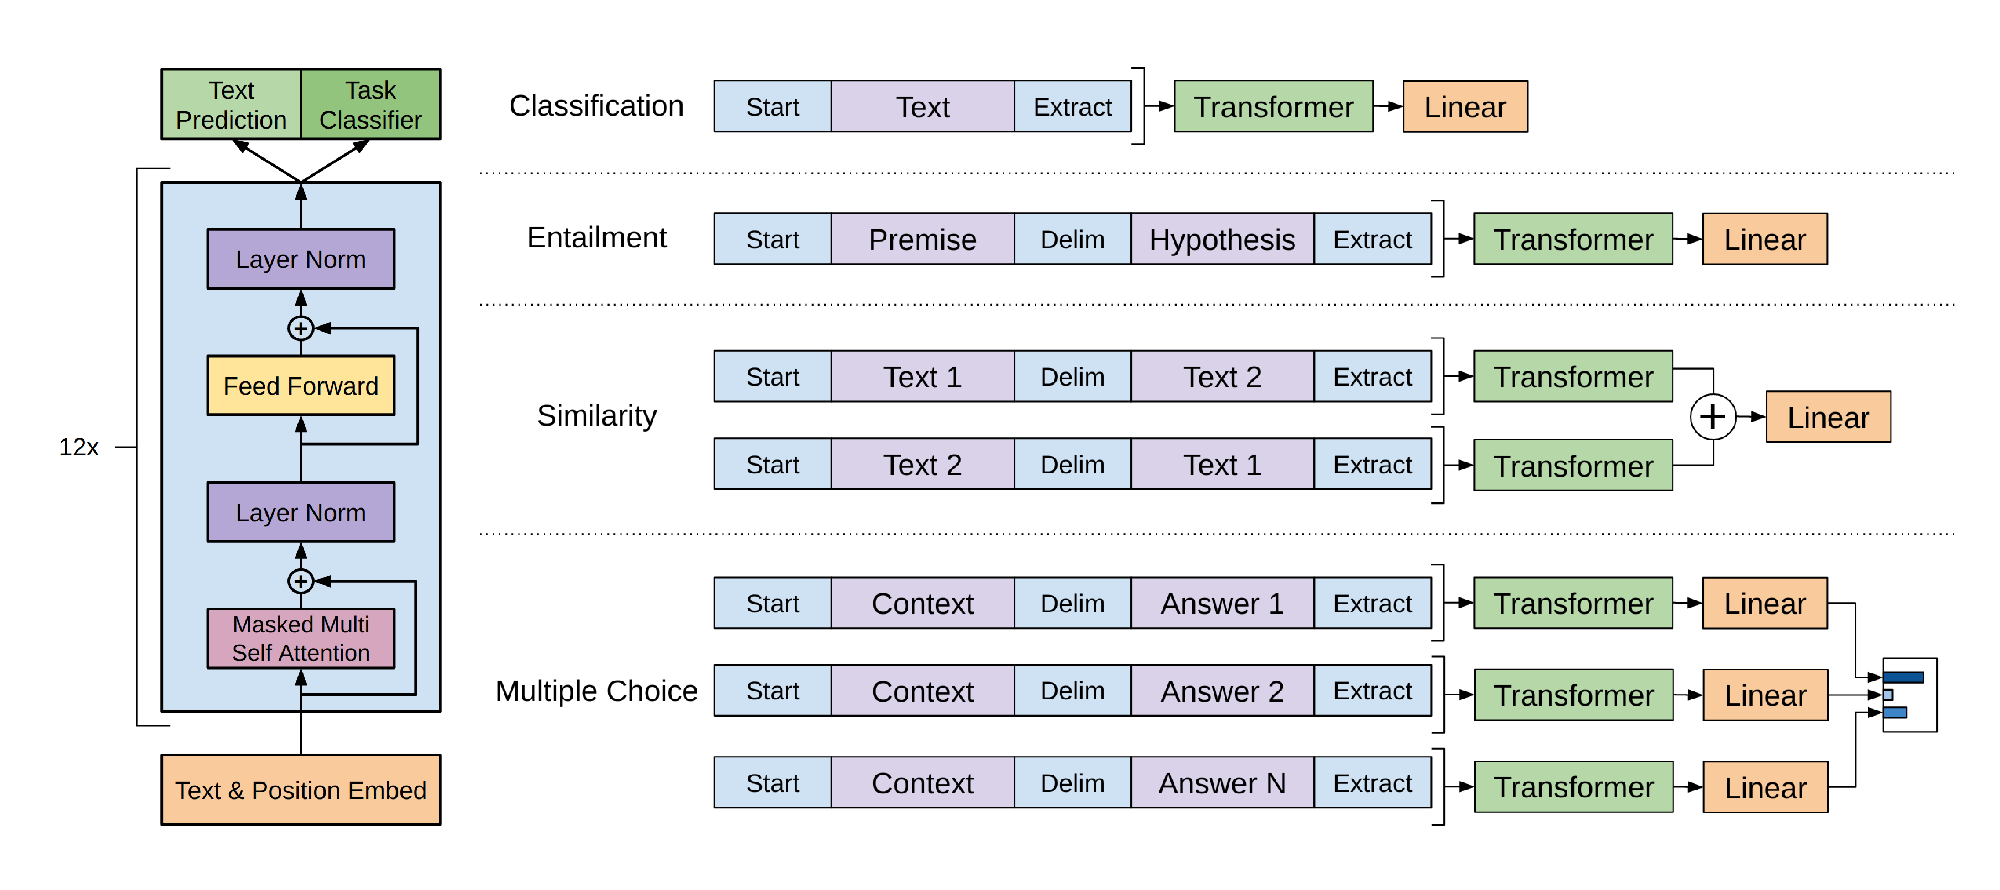
\includegraphics[width=\linewidth,pagebox=cropbox,clip]{figures/fig_gpt.pdf}
    \caption{左: GPT-2のベース手法(GPT)で使われるTransformerのモデル図,右: GPTによる自然言語処理タスクの流れ\cite{radford2018improving}.}
    \label{fig:gpt}
\end{figure}

\begin{figure}
    \centering
    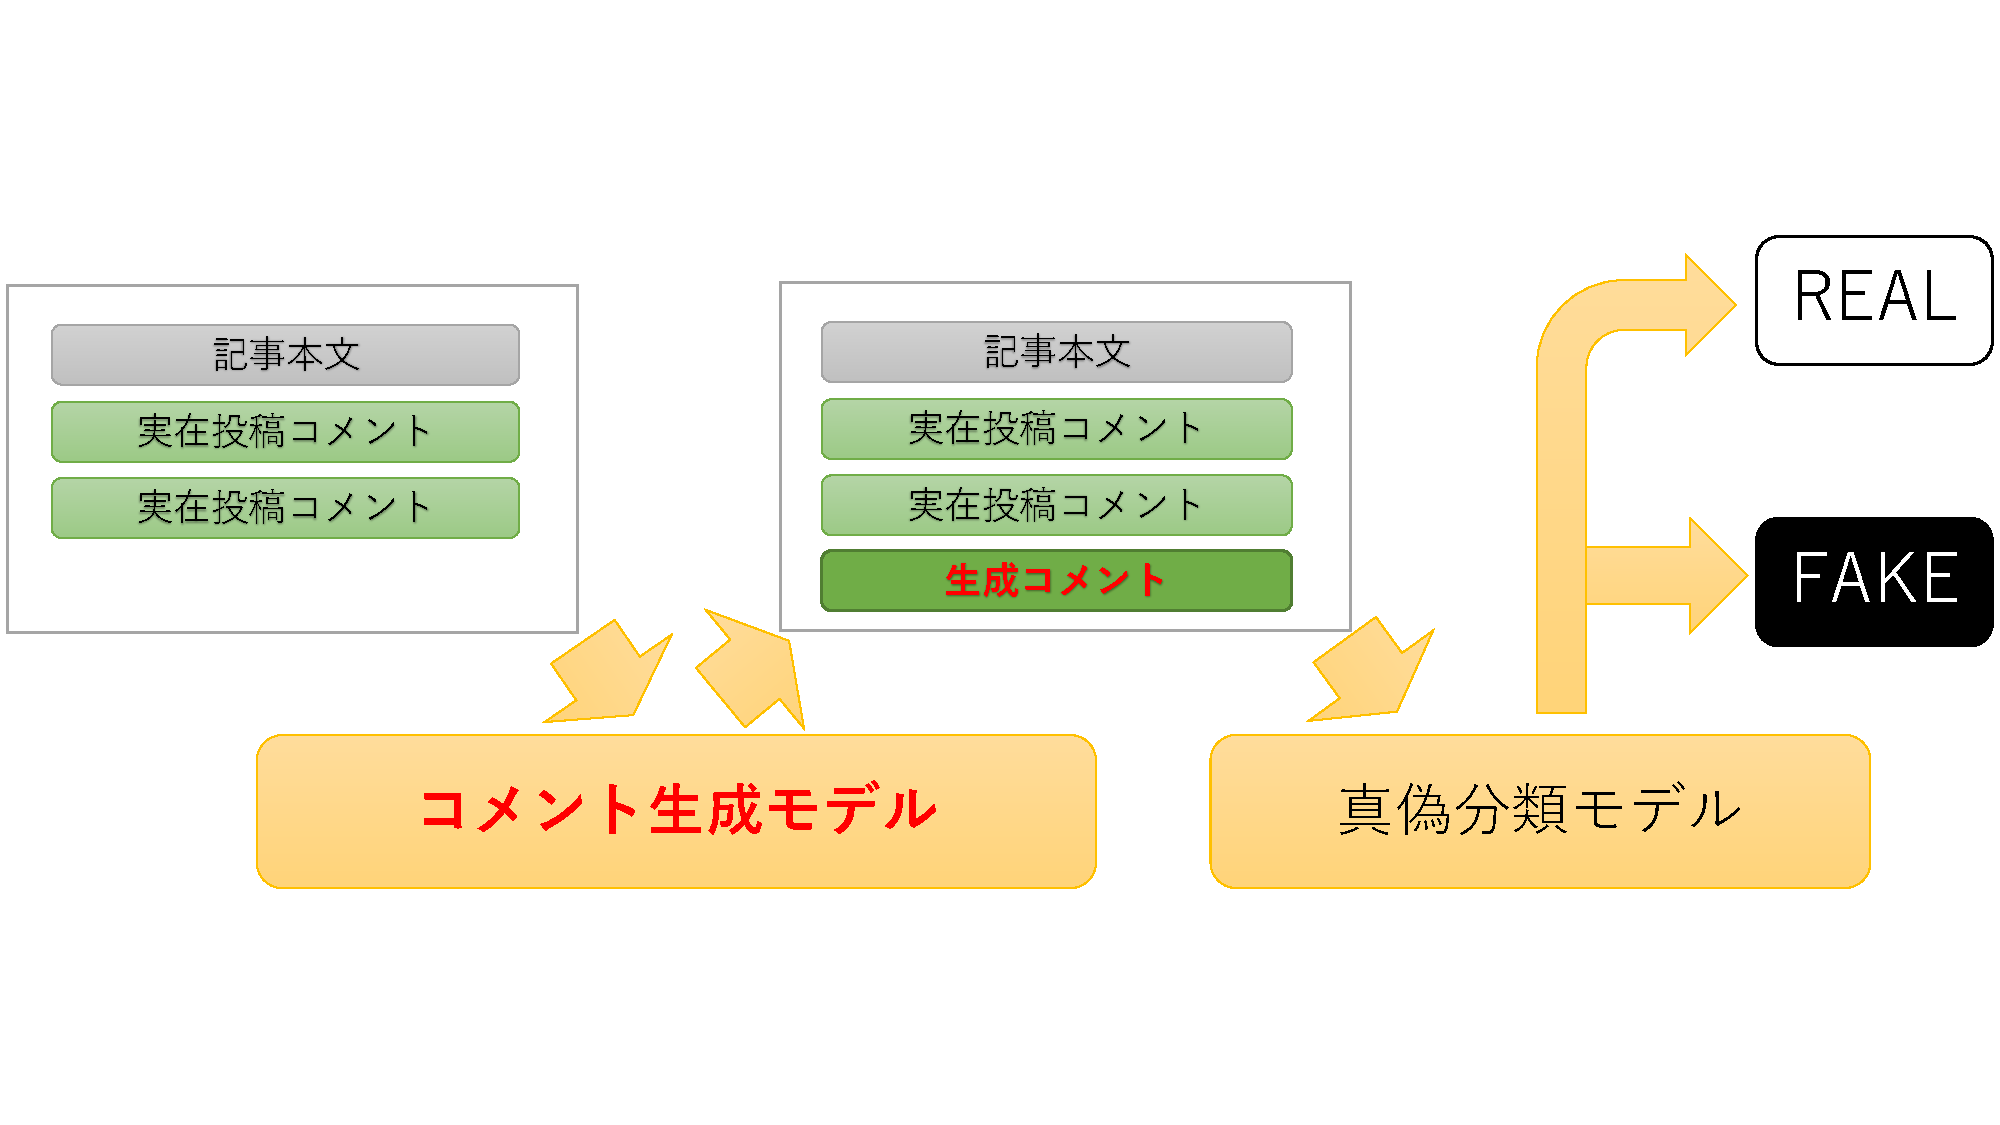
\includegraphics[width=\linewidth,pagebox=cropbox,clip]{figures/fig_model.pdf}
    \caption{モデルの概要図}
    \label{fig:model}
\end{figure}

\begin{figure}[h]
    \centering
    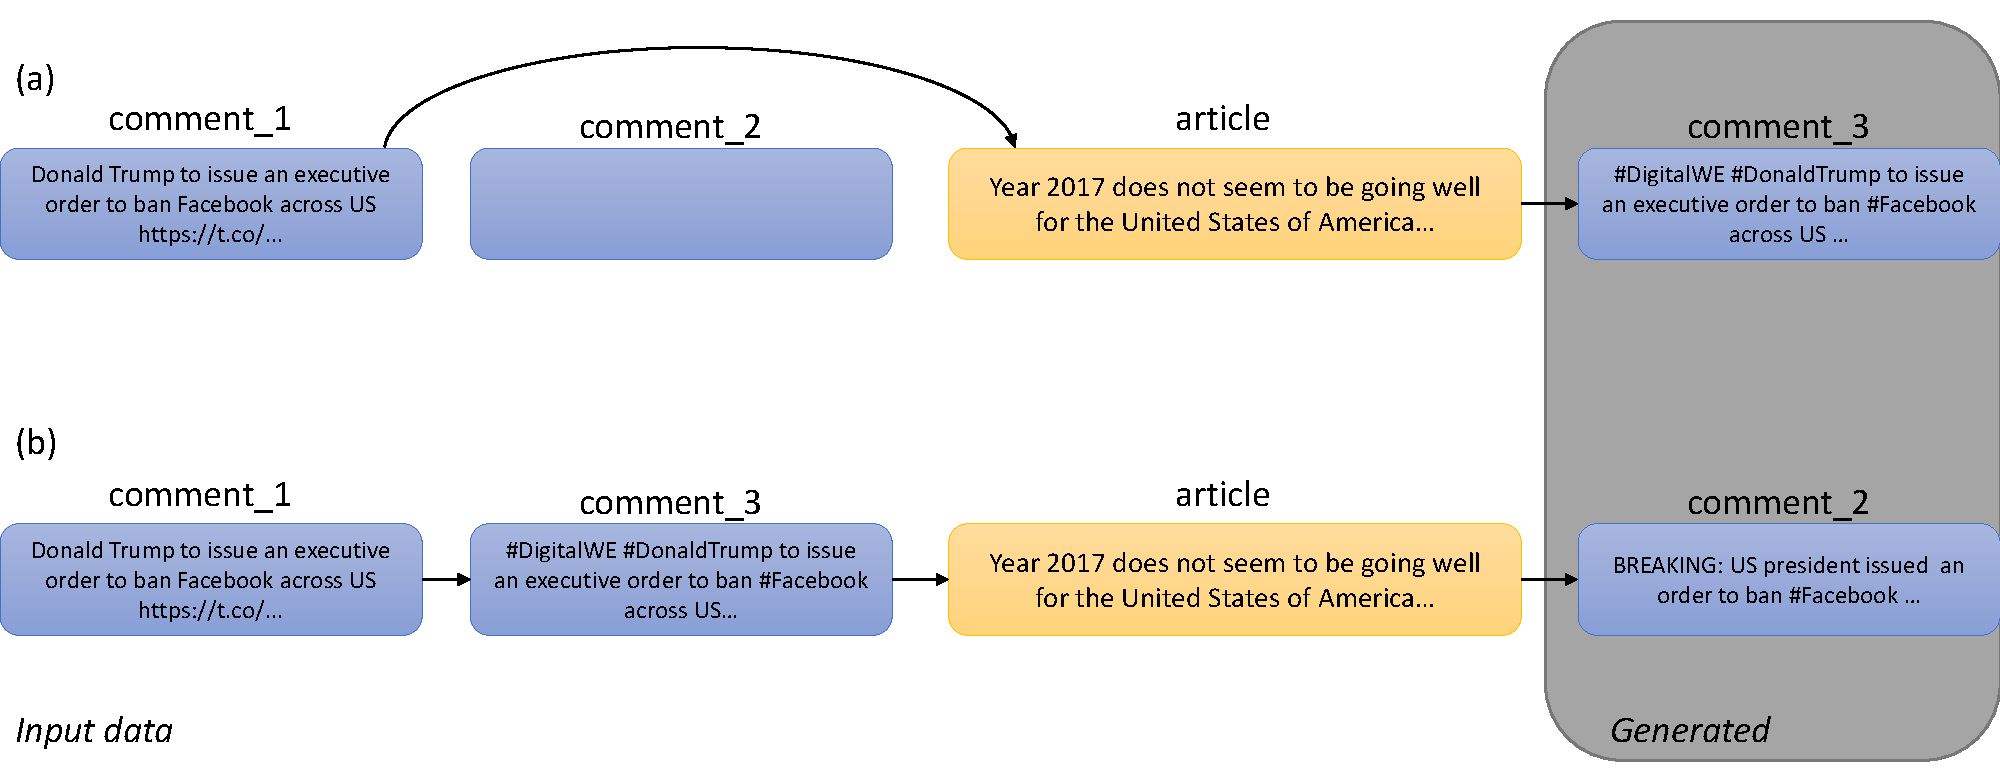
\includegraphics[width=\linewidth,pagebox=cropbox,clip]{figures/fig_method.pdf}
    \caption{
        提案モデルのコメント生成例.
        (a)は記事と1件の実際に寄せられたコメントからコメントを生成している.
        (b)は(a)で生成したコメントを含めた状況で更にコメントを生成している.
    }
    \label{fig:method}
\end{figure}

\begin{figure}[t]
    \centering
    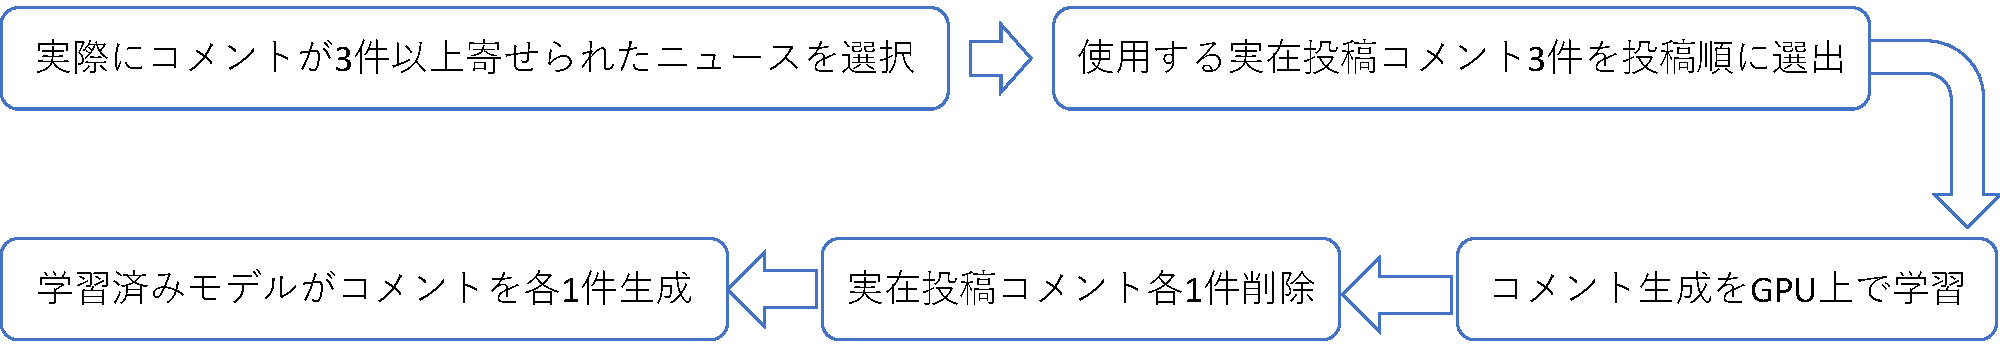
\includegraphics[width=\linewidth,pagebox=cropbox,clip]{figures/fig_process.pdf}
    \caption{実験の流れ}
    \label{fig:process}
\end{figure}

\begin{algorithm}[h]
    \caption{提案モデルが行うコメント生成学習の流れ}
    \label{alg:generate}
    \begin{algorithmic}[1]
%        \REQUIRE $A = \{a_1, a_2, ..., a_n\}, C_A = \{c_{a_1}, c_{a_2}, ..., c_{a_n}\}$
%        \ENSURE $\hat{c_{a_{i3}}}$
        \Procedure{Prepare-Generate}{$A, C_A$}
            \For {$i=1 \, \ldots \, N$}
                \State{articleRand $=$ a random float number between 0 to 1}
                \State{commentRands $=$ three random float numbers between 0 to 1}
                \If{articleRand $\leq 0.35$}
                    \State{make $a_i$ empty}
                \EndIf
                \For {$j=1 \, \ldots \, 3$}
                    \If{articleRand[j] $\leq 0.1$}
                        \State{make $c_{a_{ij}}$ empty}
                    \EndIf
                \EndFor
            \EndFor
        \EndProcedure

        \Procedure{Generate-Training}{$A, C_A$}
            \For {$i=1 \, \ldots \, \mathrm{maxEpoch}$}
                \For{$i=1 \, \ldots \, N$}
                    \While{empty element in $\{a_i, c_{a_i}\}$}
                        \State{Fill an element which is empty in $\{a_i, c_{a_i}\}$}
                    \EndWhile
                \EndFor
            \EndFor
        \EndProcedure
    \end{algorithmic}
\end{algorithm}

\begin{algorithm}
    \caption{提案モデルが行うコメント生成を伴う真偽分類を行う際の流れ}
    \label{alg:classify}
    \begin{algorithmic}[1]
        \Procedure{Classify}{$A, C'_A$}
            \For{$i=1 \, \ldots \, N$}
                \State{Add \texttt{[CLS]} in tail of set ($a_i, C'_{a_i}$)}
                \State{\texttt{[CLS]} has features of set ($a_i, C'_{a_i}$)}
                \State{Classifier outputs label $\hat{y}$ from the \texttt{[CLS]}}
            \EndFor
        \EndProcedure
    \end{algorithmic}
\end{algorithm}


\section{実験}\label{sec:gen_exp}
この章では,提案手法の有効性を検証するために行った実験と結果について記述する.

\subsection{データセット}
\label{sec:dataset}
記事とそれに寄せられたコメントをもつデータセットとしてFakeNewsNet\cite{Shu2018FakeNewsNetAD}を採用した.
これはファクトチェックプラットフォームであるPolitiFact(政治ニュース専門)とGossipCop(芸能ニュース専門)によりファクトチェック(真偽ラベル付けも兼ねる)が行われた記事の内容と,それにTwitter上で寄せられたコメント投稿等を持っている.

実験に先立ち,今回のモデルの構造上少なくとも3件コメントが寄せられているニュースである必要がある他,そのいずれも英文で書かれたコメントである記事とコメントのセットを選出した.
表\ref{tbl:dataset}の通り今回,PolitiFactを使用した実験ではReal・Fakeで各200セット,GossipCopでは各ラベル毎に2000セット使用した.

\begin{table}[h]
    \caption{実験で使用したラベル毎のデータセット内容.記事数・コメント数はRealとFakeともに同数である.}
    \label{tbl:dataset}
    \centering
    \begin{tabular}{lcc}
        \hline
        ファクトチェックプラットフォーム     & 記事数 & コメント数 \\ \hline
        PolitiFact & 200   & 600   \\
        GossipCop  & 2000  & 6000  \\ \hline
    \end{tabular}
\end{table}

\subsection{実験内容}
\label{sec:exp_contents}
今回実験を2種類行った.

\subsubsection{真偽分類成績調査}
生成コメントを追加することによって真偽分類の傾向に変化がみられるか調べた.
比較対象として2件ともにデータセットがもつコメントを使用したものと,コメントを使わず記事内容のみで真偽分類したものを用意した.
この実験にはセット数が多く汎化性が高いGossipCopにファクトチェックされた記事を採用した.
また、PolitiFactにファクトチェックされた記事を採用した場合の結果も調べた。

\subsubsection{生成コメント傾向調査}
生成されたコメントは真偽でどのような単語の傾向が現れるか調べた.
傾向の違いを調べることによって,拡散の初期段階において読者が記事をどう捉えているのか知ることができる.
この実験はセット数が少ないが社会に与える影響が芸能に比べて大きくなりやすい政治ニュースを扱うPolitiFactにファクトチェックされた記事を採用した.

実際に生成されたコメントに対して,すべてアルファベットを小文字にした上で単語ごとの出現回数と出現確率を算出した.
また,算出するにあたって記号(クォーテーションやピリオド,コンマなど)やURLの削除を行ったほか,``a''や``is''といったストップワードはNLTK\cite{bird-loper-2004-nltk}が提供するメソッドを使用して除外した.
なお,コメントの収集元がTwitterであることから,Twitter独自の用法をもつ記号(ハッシュタグ\#やメンション@),またコロンは例外として除外しなかった.

\section{実験結果}
\label{sec:result}
GossipCopを対象とした真偽分類実験結果は表\ref{tbl:classify_results}の通りである.
提案モデルは再現率において全体ベストとなったものの,適合率においては生成モデルを使わない方が優秀であることが読み取れる.

分類において生成コメントの有無によって真偽が覆った回数も調査した.その結果が表\ref{tbl:reversed}の通りである.

また,表\ref{tbl:generated_comments}の生成されたコメントの例のように,生成コメントには文法面にさらなる改善の必要性が残された.

PolitiFactを対象とした真偽分類実験結果は表\ref{tbl:classify_results_pf}の通りである.
提案モデルはいずれの指標において、全体ベストを示した.

PolitiFactを対象とした生成コメントの出現割合では,以下のような傾向が見られた.
\begin{itemize}
    \item 真偽問わず最も頻度が高い単語は``via''であり,真偽全体の単語のうち約1.5\%を占めた.
    \item それに続いて``trump''と``obama''が続いたが,いずれも割合は1\%を下回った.
\end{itemize}

これに加えて,真偽における傾向差として以下の違いが見られた.

\begin{itemize}
    \item ``via''は真偽単独で見てもそれぞれで最も高い頻度で生成されていた.
    \item 偽における``via''の生成頻度は正しい場合に比べて約2倍であり,その差は約0.9ポイントと偽頻出上位10単語中最多だった.
    \item ``breaking:''という単語が``via''に次いで2番目に頻度の差が高い単語であり,その差は0.7ポイントだった.
\end{itemize}


\begin{table}
    \renewcommand{\arraystretch}{1.3}
    \caption{GossipCopデータセットにおける分類成績}
    \label{tbl:classify_results}
    \centering
    \begin{tabular}{lccc}
        \hline
        入力データ           & 適合率 & 再現率 & F値 \\ \hline
        記事本文のみ         & 0.647     & 0.615  & 0.631    \\
        + 実在コメント2件  & \textbf{0.774}     & 0.635  & \textbf{0.698}    \\
        + 生成コメント1件 & 0.626     & \textbf{0.695}  & 0.659    \\ \hline
    \end{tabular}
\end{table}

\begin{table}
    \caption{GossipCopデータセットにおける生成コメントの追加によって真偽が覆った件数}
    \label{tbl:reversed}
    \centering
    \begin{tabular}{llccc} \hline
        正解ラベル & 覆ったパターン & 覆った件数 & 覆らなかった件数 & 覆った割合[\%]\\ \hline
        \multirow{2}{*}{Real} & Real $\rightarrow$ Fake & 60 & 103 & 37\\
                              & Fake $\rightarrow$ Real & 14 & 23 & 38\\ \hline
        \multirow{2}{*}{Fake} & Real $\rightarrow$ Fake & 35 & 38 & 48\\
                              & Fake $\rightarrow$ Real & 23 & 104 & 18\\ \hline
    \end{tabular}
\end{table}

\begin{table}
    \renewcommand{\arraystretch}{1.3}
    \caption{PolitiFactデータセットにおける分類成績}
    \label{tbl:classify_results_pf}
    \centering
    \begin{tabular}{lccc}
        \hline
        入力データ           & 適合率 & 再現率 & F値 \\ \hline
        記事本文のみ         & 0.793     & 0.851  & 0.821  \\
        + 実在コメント2件  & 0.897 & 0.839 & 0.867 \\
        + 生成コメント1件 & \textbf{0.909}     & \textbf{0.968}  & \textbf{0.938}   \\ \hline
    \end{tabular}
\end{table}

\begin{table}
    \caption{PolitiFactデータセットにおけるラベル別の生成コメント内の頻出単語}
    \label{tbl:frequency}
    \centering
    \begin{tabular}[]{llc}\hline
        順位&Realの頻出単語&出現率[\%]\\ \hline
        \rownumber & via & 1.07 \\
        \rownumber & trump & 0.69 \\
        \rownumber & obama & 0.55 \\
        \rownumber & new & 0.41 \\
        \rownumber & national & 0.41 \\
        \rownumber & said & 0.38 \\
        \rownumber & news & 0.38 \\
        \rownumber & clinton & 0.31 \\ \hline
    \end{tabular}
    \quad
    \begin{tabular}[]{llc}\hline
        順位&Fakeの頻出単語&出現率[\%]\\ \hline
        \rownumber & via & 2.03 \\
        \rownumber & trump & 0.97 \\
        \rownumber & \textbf{breaking:} & 0.92 \\
        \rownumber & obama & 0.87 \\
        \rownumber & president & 0.73 \\
        \rownumber & united & 0.53 \\
        \rownumber & states & 0.44 \\
        \rownumber & years & 0.39 \\ \hline
    \end{tabular}
        
\end{table}

% \begin{landscape}
\begin{table}[h]
    \caption{実際に生成されたコメントの一部の冒頭."\textbackslash n"は改行記号である.}
    \label{tbl:generated_comments}
    \centering
    \begin{tabular}{ll}
        \hline
        ラベル & 生成コメント(冒頭) \\ \hline
        \multirow{2}{*}{Real} & \texttt{talks to theWa at theus\textbackslash n�,}\\
        & \texttt{Read,rin would Huck Randall. didn}...\\\hline
        \multirow{2}{*}{Real} & \texttt{accuracy!co/g Making,} ...\\
        & \texttt{single change of Wyn, the fell Featuresogue,}\\\hline
        \multirow{2}{*}{Real} & \texttt{Vi thepressBir 143 Introdu}\\
        & \texttt{sting Sullivan remarksregnancy prof}...\\\hline
        \multirow{2}{*}{Real} & \texttt{she theheyhl height backyardGame}\\
        & \texttt{his-Whereas to peach THRrd, go}...\\\hline
        \multirow{2}{*}{Real} & \texttt{gory for Emil-----][PU}\\ & \texttt{Adidasolan Song and Patrick.itans.\textbackslash n\textbackslash n}...\\ \hline\hline
        \multirow{2}{*}{Fake} & \texttt{guest Chelsea1p henEach}\\
        & \texttt{psychologicalZEinspired second resort}...\\\hline
        \multirow{2}{*}{Fake} & \texttt{eeleurg, Rum rates as aHS Army}\\
        & \texttt{to week it3 transplant nomination KnW}... \\\hline
        \multirow{2}{*}{Fake} & \texttt{View was22 the Ridge caval Shar}\\
        & \texttt{silicone Copyright warm Yourhm Had,}...\\\hline
        \multirow{2}{*}{Fake} & \texttt{\textbackslash n\textbackslash n\textbackslash n\textbackslash n\textbackslash n\textbackslash nThe756 anticipating}\\
        & \texttt{appetite sungIMels sightings in}...\\\hline
        \multirow{2}{*}{Fake} & \texttt{s tagging going.What back advocate}\\
        & \texttt{Rum to- lonelymentation her tie}...\\ \hline
    \end{tabular}
\end{table}
% \end{landscape}

\section{考察}\label{sec:gen_evl}
\subsection{真偽分類成績指標}
\label{sec:classify_index}
\cref{tbl:classify_results}が真偽分類を行った結果である.
GossipCopデータセットにおいては、記事のみから分類した場合と,記事に加えてコメントを入力に含めた場合では,コメントを含めると分類成績に改善がみられることがわかる.
このことから,記事単体に加えて読者が送ったコメントが正確な真偽分類に貢献することが示されている.

また実在コメントのみ入力した場合と,加えて提案モデルによって生成したコメントを含めた場合より,提案モデルは再現率は全体ベストを示したものの,適合率に大きな課題を残した.
これは提案モデルがソーシャルコンテキストが制限されている状況でも,単純に真偽分類を行うより多くの偽情報の検出ができることを意味する.

また、PolitiFactとGossipCopといったファクトチェックプラットフォームによる傾向の差異は、扱われるニューストピックの違いによるものと考えられる。
具体的には、政治的主張の場合は公的機関や一次情報といった明確な情報源と照らし合わせやすい影響から、コメントによる指摘が発生しやすいといった要因が考えられる。

\subsection{真偽分類傾向差の比較}
\label{sec:classify_trend}
実際真偽分類の傾向を調べるため,Realを0,Fakeを1とした分類の平均値を調べた.
その結果生成コメントがない場合は0.41,ある場合は0.55で,対応ありt検定の結果$p<0.05$だった.
このことから,生成コメントによってFakeを多く分類する傾向の有意差がみられた.
また\cref{tbl:reversed}より,生成コメントがない場合でRealと判定していた検出モデルが,
生成コメントの追加によってFakeへ判断が95件覆っていることが読み取れる.
内訳では95件中35件が正解ラベルがFakeである偽情報であることと,
正解ラベルFakeのうち23件のみ生成コメントでFakeからRealに覆っていることから,
生成コメントの追加によって検出モデルがRealと誤って判断しにくくなったことが伺える.
このことは正解ラベル毎に生成コメントによって出力ラベルが覆った件数を生成コメントの出力ラベル毎の件数で割った割合からも,
特に正解ラベルFakeの場合においてモデルが騙されにくくなったとみられる.
一方残りの60件はRealに対してFakeと誤った判断へ誘導しているため,
生成コメントによる適合率の減少を誘発していると考えられる.

また生成コメントなしの出力ラベルに対して,
真偽が覆った件数を、元々の出力ラベル毎に分けた件数分無作為にラベルを反転させた時の
分類指標を調べたところ,適合率は0.486, 再現率は0.390, F値は0.429といずれの手法を大幅に下回っていた.

\cref{sec:classify_index}と併せると,この傾向はファクトチェックが必要なニュースを探す際に役立つことを示唆している.
ただし適合率が低く他のモデルより多く正しいニュースを偽情報として誤って検出するため,改善が求められる.
今後は,より多くのデータセットを用いた場合に傾向が変化するか調べる必要がある.

\subsection{単語生成傾向}
コメント生成の傾向から,提案モデルは入力されたニュース記事が扱うトピックの学習に成功したように見える.
生成されたコメントの多くが政治的内容を含むものが多かった理由として,データセットが扱う内容の影響を受けたことが考えられる.

生成コメントの中で興味深い単語は``breaking:''である.
この単語は偽情報に寄せられたコメントとして生成されていた.
本研究と同じくコメントとして尤もらしい単語を生成するTCNN-URG \cite{ijcai2018-533}でも,
偽を示すシグナルとして``!''や``?'',そして``false''が報告されていたが,``breaking:''は報告されていなかった.
よって,この``breaking:''も偽情報を示す重要なシグナルである可能性がある.

\subsection{生成コメントの内容}
生成されたコメントは文法面に改善点が残されているが,これはデータセットの規模不足が原因として考えられる.
Groverモデルは120GBにも及ぶニュースデータセットから訓練されていた \cite{DBLP:journals/corr/abs-1905-12616}ことも考慮すると,
改善のためにはさらなる追加データを収集する必要がある可能性が示されている.

もう1つの文法面の完成度改善に向けて考えられる対策として,ベースとなる手法の変更も考えられる.
\cref{sec:method_overall}の通り,提案手法はGPT-2から発展させたものである.
現在ではGPT-2の発展型にあたるGPT-3\cite{brown2020language}やGPT-4 \cite{openai2023gpt4}を始めとする自然言語処理モデルの進歩が著しいため,
ベースとなるモデルを変更することでより自然なコメント生成が可能となる可能性がある.

\cleardoublepage
\chapter{発話内容を考慮した偽音声検出}\label{ch:spc_cnt}
\section{目的}\label{sec:cnt_pur}
\subsection{形式の位置づけ}
音声を入力とする話者認識(Speaker Recognition)には、話者識別(Speaker Identification)と話者照合(Speaker Verification)という2種類の形式がある \cite{FURUI1997859,628714,5745552}。
\cref{fig:speaker_recog}は2種類の形式の違いを示す。

\begin{figure}[p]
    \centering
    \begin{minipage}{0.9\linewidth}
        \centering
        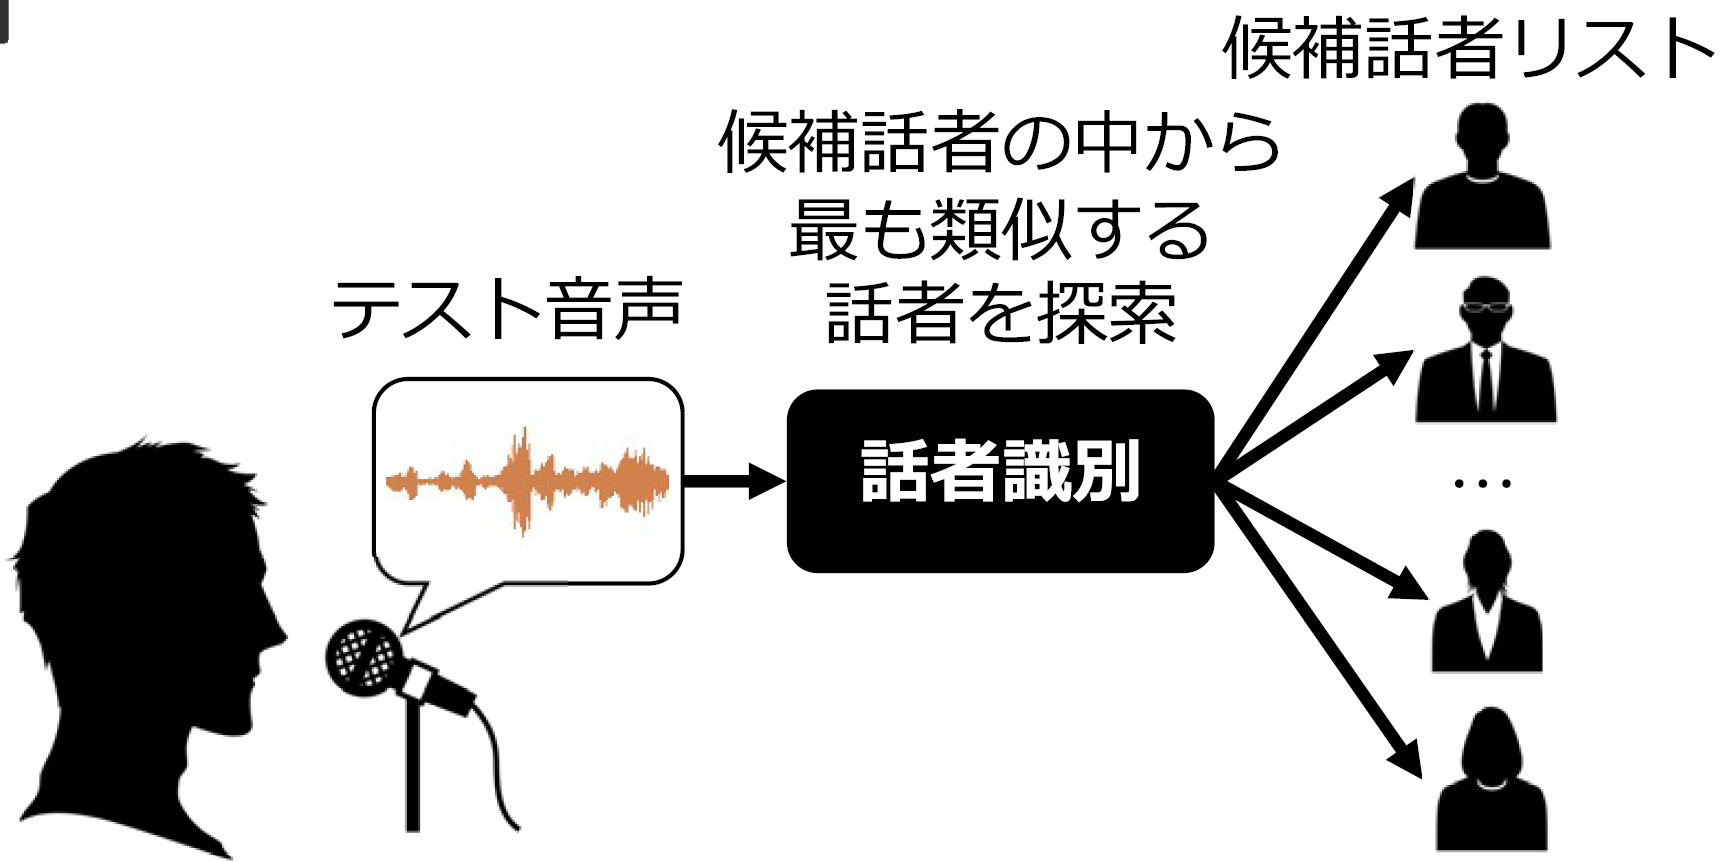
\includegraphics[width=0.8\linewidth]{figures/sd.png}
        \subcaption{話者識別}
    \end{minipage}
    \begin{minipage}{0.9\linewidth}
        \centering
        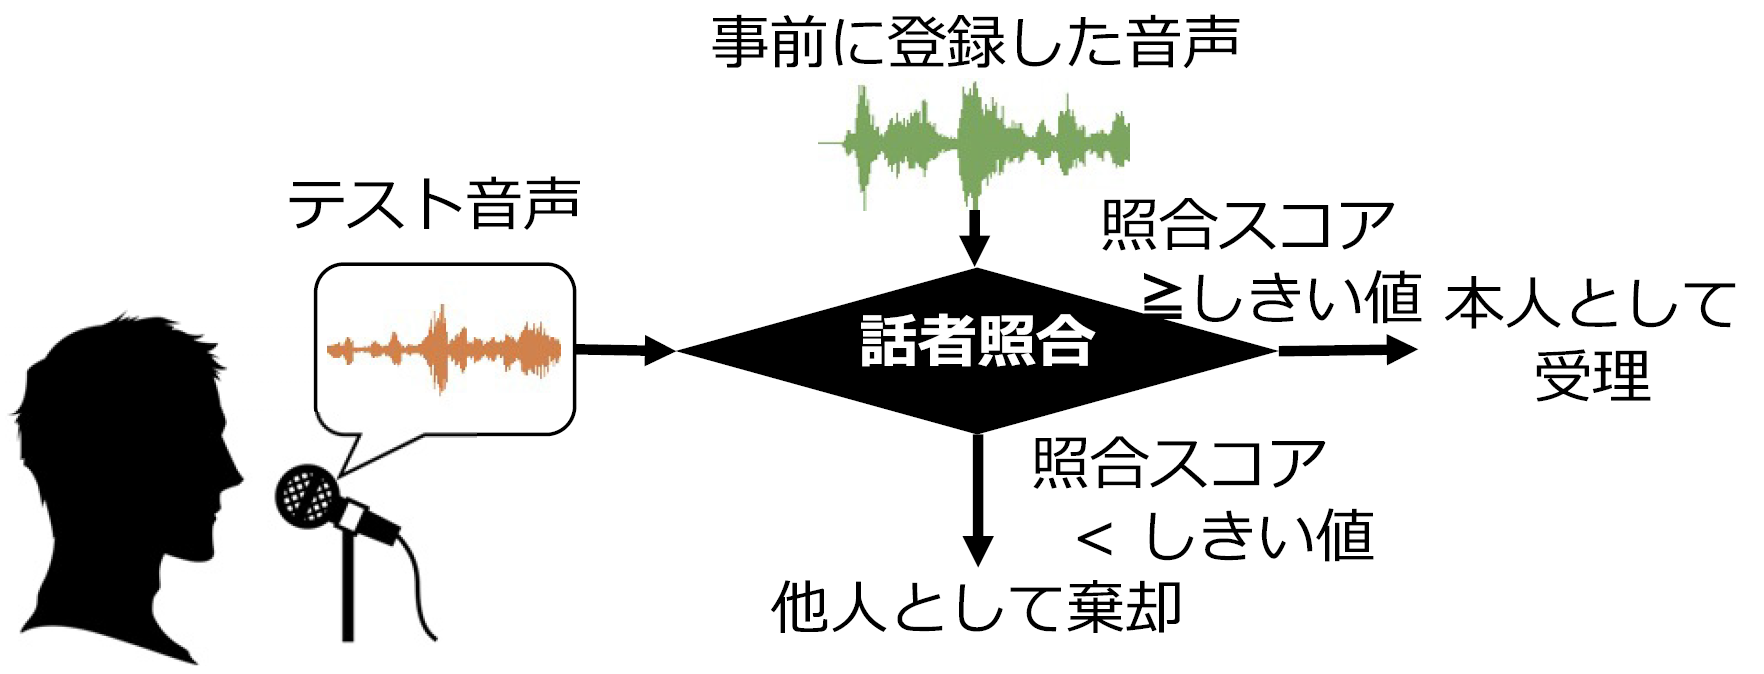
\includegraphics[width=0.8\linewidth]{figures/sv.png}
        \subcaption{話者照合}
    \end{minipage}
    \caption{話者認識の形式 \cite{俵直弘2022}}
    \label{fig:speaker_recog}
\end{figure}

話者識別は事前に登録した複数の候補者の中から提示された音声の話者を探索する1対nの推定問題であるのに対し、
話者照合では,提示された二つの音声が同一話者によるものか否かを推定する1対1の照合問題として定義する \cite{俵直弘2022}。
識別では、未知の話者を既知の話者のデータベースと比較し、最もよく一致する話者を識別結果として与える。
一方で照合では、音声サンプルが主張された人物によって話されたかどうかを判断するタスクと言える \cite{1561284}。
よって、本研究で行うなりすまし偽音声の検出は、話者照合に該当する。

また,話者認識は,登録時と照合時で同じ内容の音声を用いるテキスト依存型(text-dependent)と,
登録時と照合時で異なる内容の音声を用いるテキスト独立型(text-independent)に分類される \cite{俵直弘2022}。
ASVspoofにおけるなりすまし検出では、テキスト依存型の形式を取っている。
読み上げる音声は本人・偽いずれも新聞記事から引用した同一の文章を読み上げているため、
実際にSNS上で偽音声による偽情報が投稿された状況から乖離がある。
よって本研究では、テキスト独立型の話者照合を行う。

\subsection{検出対象の位置付け}
本研究の目的は、偽情報を話すなりすまし音声(偽音声)を自動で検出することである。
偽情報を話す偽音声には内容の確からしさと音声そのものの本人性という2種類の概念をもつ。
話す内容の確からしさは、事実か・偽情報かの2種がある。
本来ではこの2種類以外に事実ではないものの意図的に発信されたものではない誤情報もあるが、本章では考慮しない。
本人性は本人が話すか・本人以外がなりすましているかの2種がある。
本人以外がなりすます場合では機械による合成処理を含まない場合(声真似等)もあるが、
意図的に社会に不安を与える行為として行われにくいと考えられるため本章では考慮しない。

よって、偽情報を話すなりすまし音声を検出する場合、モデルへ入力する対象は内容の確からしさと本人性から以下の4種類が挙げられる。

\begin{itemize}
    \item 偽情報を話すなりすまし音声(検出したい対象)
    \item 事実を話すなりすまし音声
    \item 偽情報を話す本人音声
    \item 事実を話す本人音声
\end{itemize}

また、\cref{fig:twoPerspective}は内容信憑性・本人性の2種類による配置を表す。

\begin{figure}[p]
    \centering
    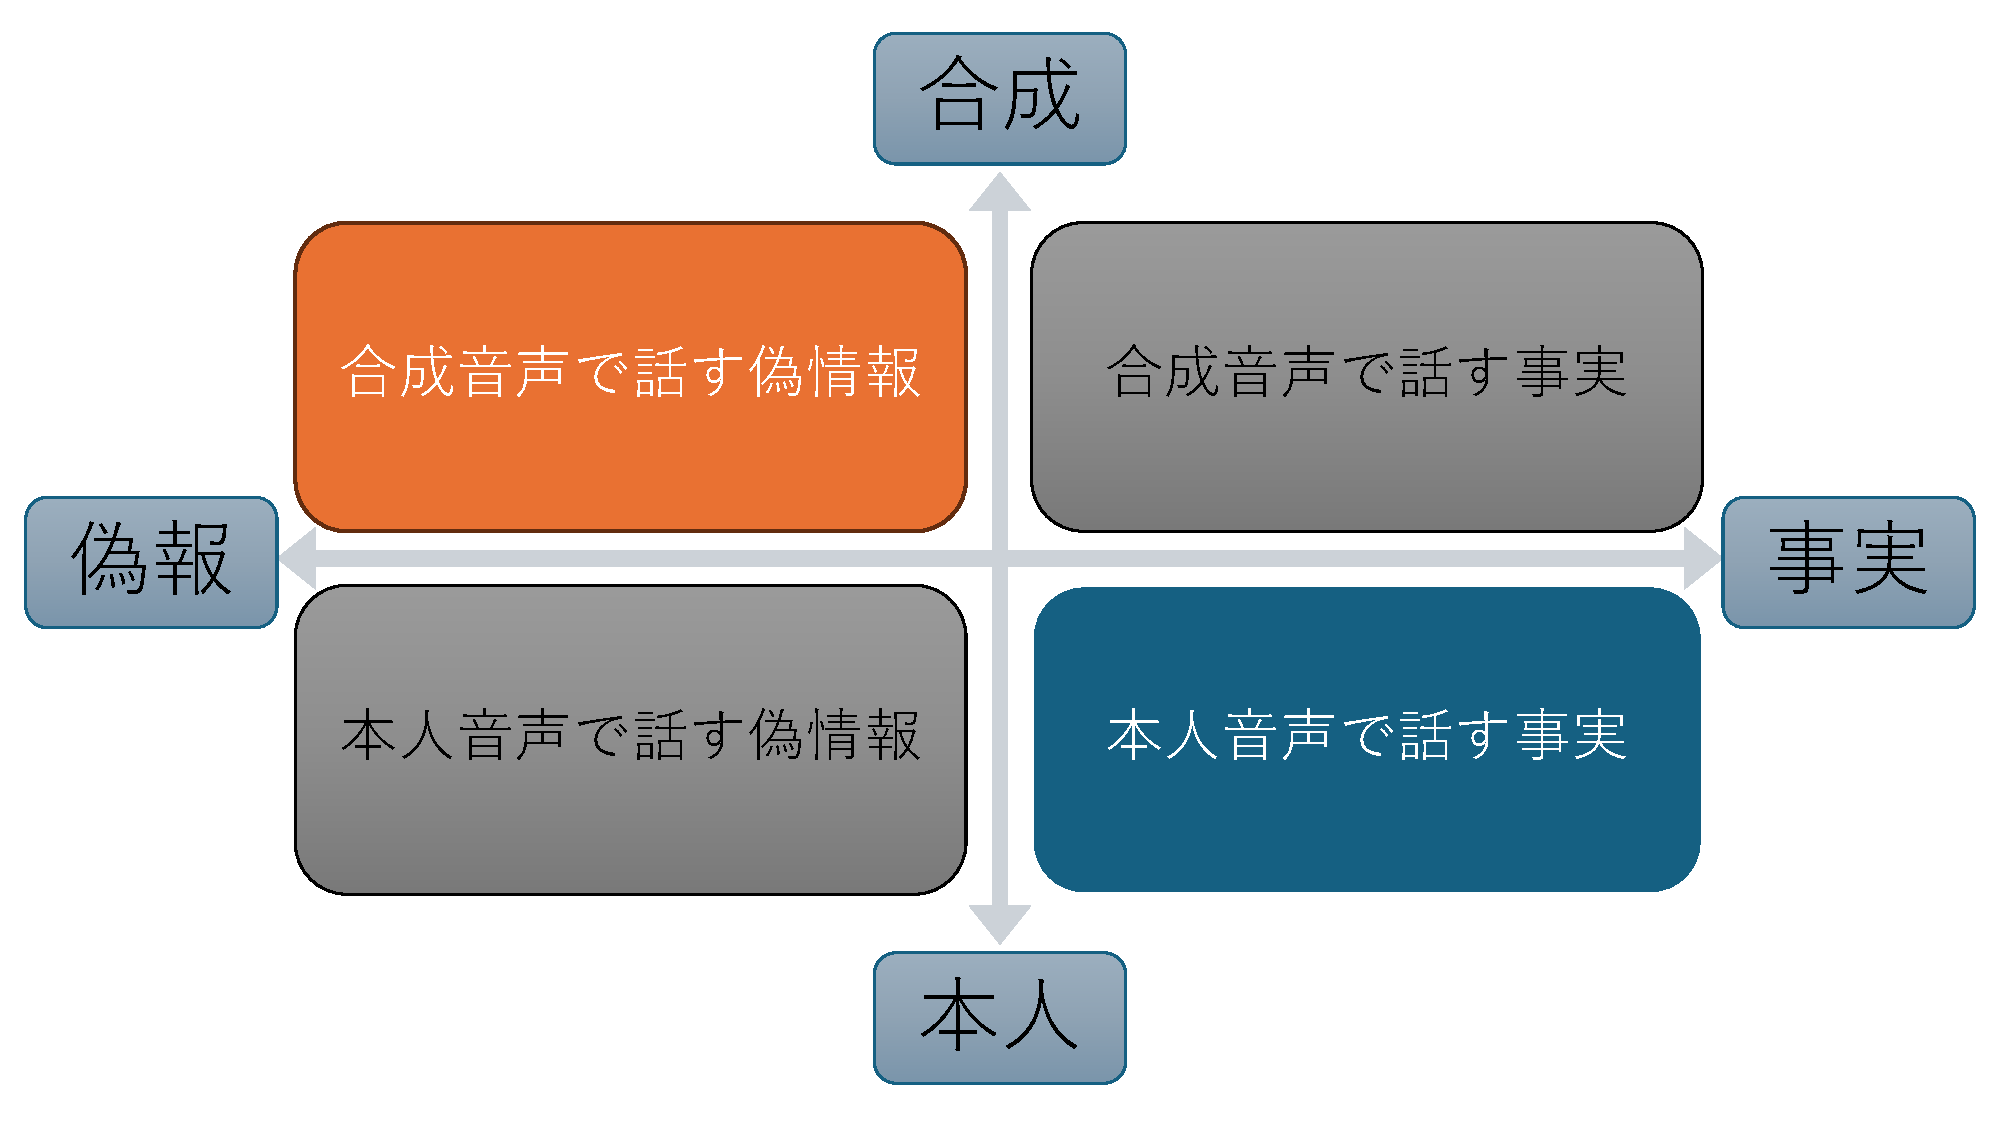
\includegraphics[width=\linewidth]{figures/D論概念図.pdf}
    \caption{発話内容の信憑性と、発話者の本人性による音声の種類。本研究では合成音声で話す偽情報と本人音声で話す事実の2種類に着目する。}
    \label{fig:twoPerspective}
\end{figure}

事実を話す本人音声は、偽情報を話すなりすまし音声とは
内容の信憑性及び本人性において、対極に位置する概念である。
本研究の予備実験では、既存手法が合成音声と本人音声を正しく識別できるかを調べるために、事実を話す本人音声を検出すべきでない対象として含めた。
%要確認

事実を話すなりすまし音声は、主にマスメディアによるニュース記事の読み上げ(AIアナウンサー)が例として挙げられる\cite{nhk2020,nhkAnnual2020}。
マスメディアによる運用が行われているため、SNS上に投稿された場合は発信者の検証で事足りる部分がある。
一方で、技術の発展によりマスメディア以外でも簡単に使えるゆえに投稿の増加も激しいと判断し、本研究での検出対象として含めた。

偽情報を話す本人音声は実際の例として演説や講演会、そして特殊詐欺などが挙げられる。
この場合は実際に話さなければならない都合上、SNS上での事例が偽情報を話すなりすまし音声に比べて変化が少ないほか、
先行研究として特殊詐欺の自動検出を目指した事例 \cite{近野恵2023}があるため、
検出したい対象に対して重要度が比較的高くないと判断し、本研究では扱わないこととした。

以上から、本研究における最終目的は事実を話す合成音声と偽情報を話すなりすまし音声の2種類の音声から検出を行うこととする。

\section{手法}\label{sec:cnt_mtd}
本節では、虚偽の主張を発信する偽音声を自動検出するための提案手法を紹介する。
我々の手法には、波形を分析する部分と、発話内容を評価する部分の2つの異なる処理部分が組み込まれている。
\cref{fig:structure}は、我々の提案する手法の構造を示している。これより各部の詳細を説明する。

\begin{figure}[p]
    \centering
    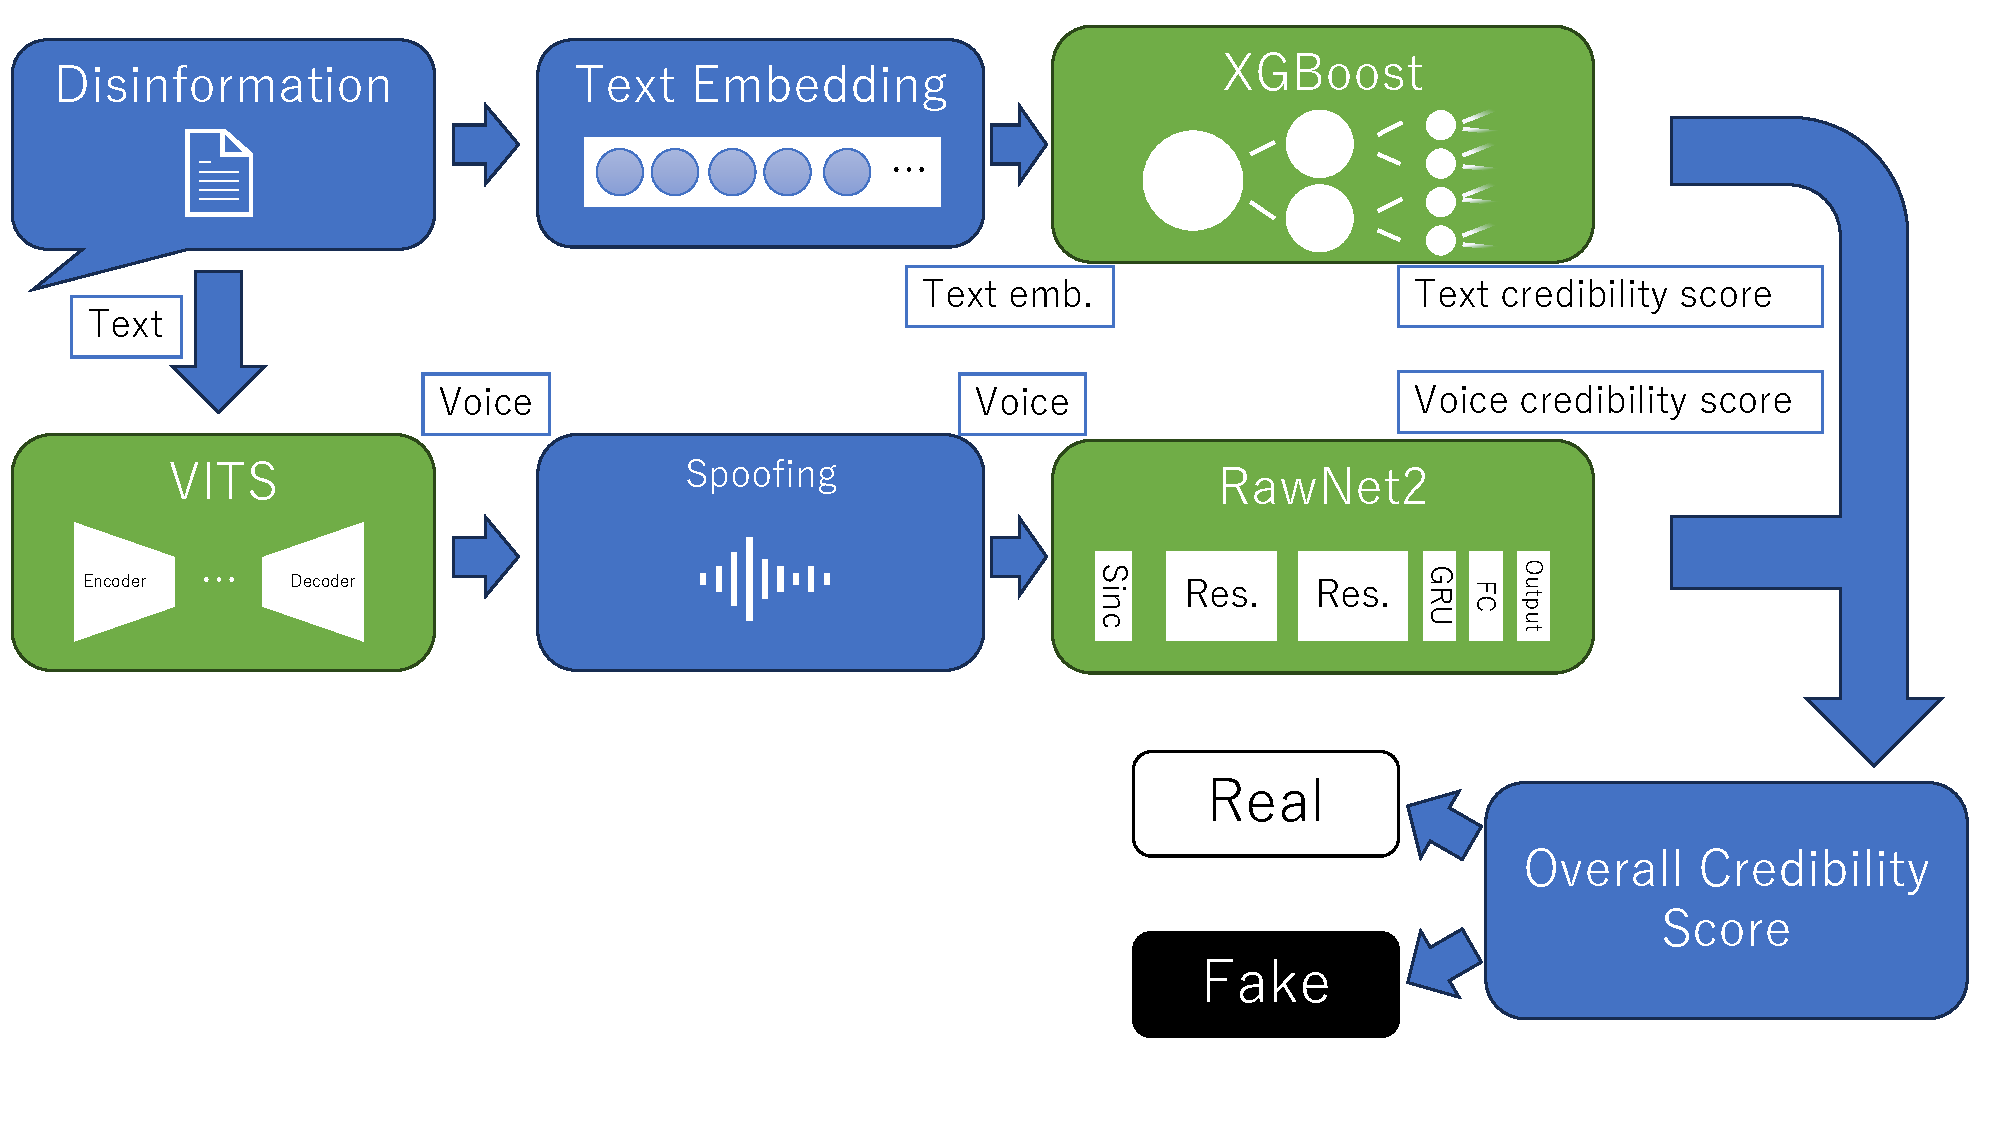
\includegraphics[width=\linewidth]{figures/Structure.pdf}
    \caption{データセットの生成から提案手法が行う分析の流れ。}
    \label{fig:structure}
\end{figure}

\subsection{波形分析}
偽音声の波形を直接分析する形式として、RawNet2とRawBoost、そして本実験ではSSL-Antispoofingを採用した。

\subsubsection{RawNet2}
音声波形を直接扱う既存手法として、
ASVspoofにてベースラインとして提供された \cite{WANG2020101114}RawNet2を採用した。
RawNet2はもともとRawNet \cite{jung19b_interspeech}から拡張された手法で、
いずれも発話レベルの特徴抽出と特徴拡張を単一モデルで完結させた上で分類を行う。
今回採用したRawNet2の構造は\cref{tb:rawnet2}の通りである。

RawNet2はRawNetモデル \cite{jung19b_interspeech}の拡張版である。
どちらのモデルも直接波形を分析して合成音声の疑いの強さを出力とするEnd-to-endの分類器として動作する \cite{jung19b_interspeech}。
RawNet2のフレームワークの最初のレイヤーは、SincNet \cite{8639585,ravanelli19_interspeech}として導入されたSinc-convolutionレイヤーを利用している。
SincNetは畳み込みニューラルネットワーク(CNN)を採用し、sinc関数に似たバンドパスフィルターを用いて入力波形をフィルターする。
第2層は残差ブロックからなり、バッチ正規化(BN)、LeakyReLU \cite{maas2013rectifier}、畳み込み層、最大値プーリング、特徴マップスケーリング(Feature Map Scaling, FMS)を含む。
FMSは \cite{woo2018cbam}で提案され、シグモイド活性化 \cite{jung20c_interspeech}を持つ注意層と同様の機能を持つ。
出力層は二値分類用に設計されており、合成によるなりすました音声と本人の音声を区別する。
このモデルは、GitHub リポジトリにある ASVspoof のベースライン設定に従って、重み付けされたカテゴリ横断エントロピーを損失関数として利用する。
これは本物の声と偽物の声を区別するための二値分類タスクであることから、本モデルの損失 $ L_{RN} $は以下の式で決定される。

\begin{equation}
    L_{RN}(y, \hat{y}) = -0.1 * y \log{\hat{y}} - 0.9 * (1-y) \log{(1-\hat{y})}
\end{equation}

この式では、$y$はラベルの値であり、$y=0$は本人に、$y=1$はなりすまし偽音声に該当する。
$\hat{y}$はRawNet2による出力に該当し、log関数にかけられている。
定数0.1及び0.9はASVspoof内での学習におけるラベル分布を根拠とする重み付けとして設定されている \cite{yamagishi21_asvspoof}。

%\begin{figure}[ht]
%    \centering
%    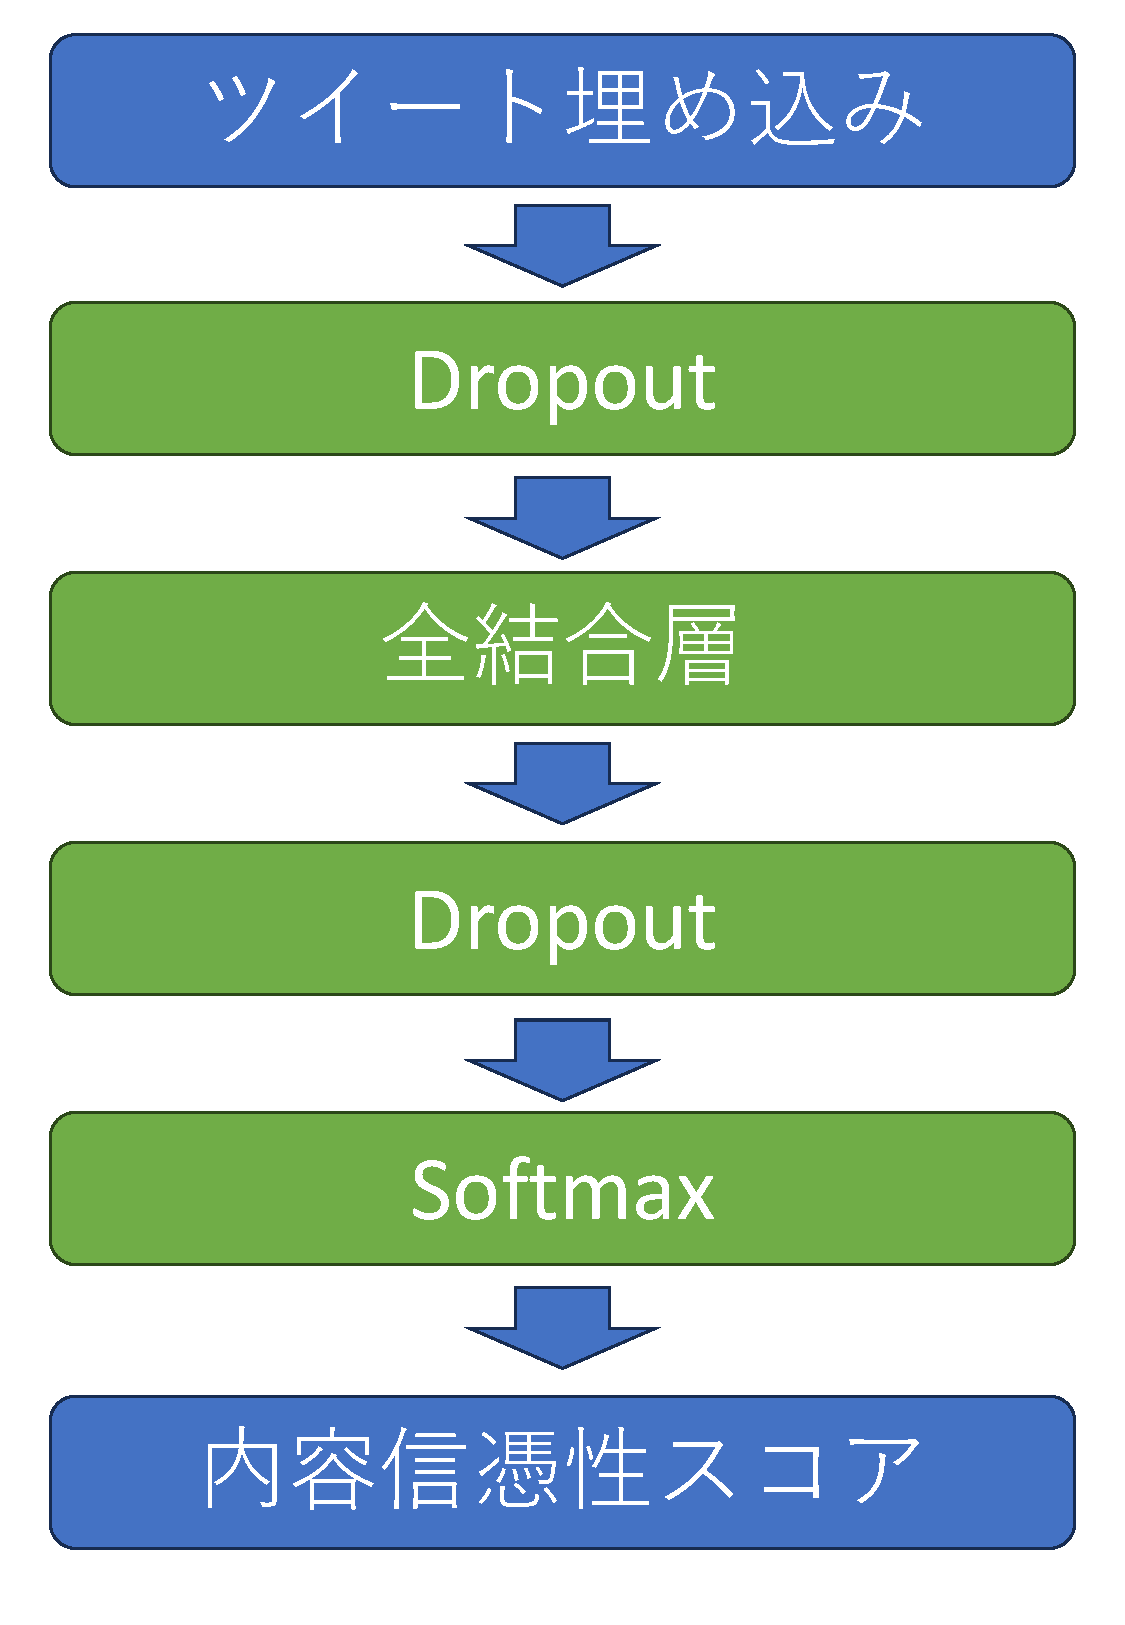
\includegraphics[width=0.5\textwidth]{./figures/ieice_nnfig.pdf} %TODO 次元情報追加
%    \caption{提案手法における内容信憑性評価部分。}
%    \label{fig:content}
%\end{figure}

\begin{table}[p]
    \centering
    \caption{ASVspoof 2019以降で採用されている \cite{9414234,yamagishi21_asvspoof}RawNet2の構造}
    \begin{tabular}{l@{}c@{}l}\hline
        層 & 入力 & 出力形式 \\\hline\hline
        \multirow{3}{*}{調整済Sincフィルタ} & 畳み込み(129,1,128) & \multirow{3}{*}{(21290, 128)}\\
        & 最大値プーリング(3) &\\
        & バッチ正規化(BN) \& LeakyReLU &\\\hline
        \multirow{6}{*}{残差ブロック}&\multirow{6}{*}{$\left\{\begin{array}{c}\rm{BN \& LeakyReLU}\\
        \rm{畳み込み(3,1,128)}\\
        \rm{BN \& LeakyReLU}\\
        \rm{畳み込み(3,1,128)}\\
        \rm{最大値プーリング(3)}\\
        \rm{特徴マップスケーリング(FMS)}\\\end{array}\right\}$}& \multirow{6}{*}{(2365, 128)}\\ \\ \\ \\ \\ \\\hline
        \multirow{6}{*}{残差ブロック}&\multirow{6}{*}{$\left\{\begin{array}{c}\rm{BN \& LeakyReLU}\\
        \rm{畳み込み(3,1,128)}\\
        \rm{BN \& LeakyReLU}\\
        \rm{畳み込み(3,1,128)}\\
        \rm{最大値プーリング(3)}\\
        \rm{FMS}\\\end{array}\right\}$}& \multirow{6}{*}{(29, 512)}\\ \\ \\ \\ \\ \\\hline
        ゲート付き回帰型ユニット&GRU(1024)&(1024)\\\hline
        全結合層&1024&(1024)\\\hline
        Output&1024&2\\\hline
        %& Maxpooling(3) &\\
    \end{tabular}
    \label{tb:rawnet2}
\end{table}

\subsubsection{RawBoost}
さらに、RawNet2とは別の手法としてRawBoost \cite{9746213}を採用した。
RawBoostは、学習にて音声内のノイズ対策として独自のデータ拡張手法を取り入れている \cite{9746213}。
このモデルを使用したのは、ASVspoofにおけるRawNet2を含むベースラインよりも良好なスコアが \cite{9746213}にて報告されたためである。
具体的なデータ拡張として、
(1)線形および非線形の畳み込みノイズ(符号化、圧縮、および送信プロセス中に導入されるノイズを再現している)、
(2)クリッピングやデバイス(マイクやアンプなど)の非最適動作などのインパルス信号依存の付加ノイズ、
(3)単一の有限インパルス応答フィルタを適用することによる定常信号非依存のノイズ付加
の3種類が導入されている \cite{9746213}。
さらに、学習時の損失関数として、GitHubリポジトリ \footnote{\url{https://github.com/TakHemlata/RawBoost-antispoofing}}で提供されている仕様に従って、同じ重み付きクロスエントロピー損失を採用した。

\subsubsection{SSL Anti-spoofing}
本実験では、SSL Anti-spoofingも導入した。
RawBoostと同じくTakら \cite{tak2022automatic}によって提案された手法である。
RawNet2との違いとして、入力を直接受ける部分がSincフィルタではなくwav2vec 2.0 \cite{NEURIPS2020_92d1e1eb}を導入し、自己教師あり学習を取り入れている。

この手法はASVspoof2021の開催後に行われた事後タスクにて参加シナリオ中で最も優秀な成績を収めている \cite{10155166}。

\subsection{埋め込みによる発話内容の分析}
音声の内容を考慮するために、MuMiNデータセット \cite{10.1145/3477495.3531744,NielsenMcConville2022}から得られる投稿埋め込みを活用する。
採用した理由として、データセット内でテキスト埋め込みが特徴としてすぐに使える点が挙げられる。
この埋め込みはBART-large-CNN \cite{lewis-etal-2020-bart}を使って生成される。
投稿埋め込み用の分類器としてXGBoost \cite{10.1145/2939672.2939785}を採用した。
今後のの計画には、ディープニューラルネットワークモデルを組み込むことが含まれている。
また、自動音声認識モデルを統合し、ソーシャ ルメディアのコンテキスト内でDeep Fakeの声を検出する包括的なアプローチを取り入れることも視野に入れている。
損失$L_{emb}$は、Chen Tら \cite{10.1145/2939672.2939785}で詳しく説明されているように、重み付き二乗損失の平均として計算され、以下のように定義される。

\begin{align} 
        L_{emb} = \sum_l (\hat{y_i}, y_i) + \sum_k \Omega (f_k) \\
        \text{where}~\Omega (f) = \gamma T + \frac{1}{2} \lambda ||w||^2
\end{align}

この式では、$y_i$は$i$番目のラベルの値を示し、$\Omega$は葉ノードの数($T$)と重みのL2ノルムからなり、正則化項として総和がモデルの複雑さにペナルティを与える \cite{10.1145/2939672.2939785}。
定数$\gamma$および$\lambda$は今回では公式ドキュメント \footnote{\url{https://xgboost.readthedocs.io/en/stable/parameter.html}}にてモデルのデフォルト値とされていた0として実装した。
つまり今回では発話内容学習による損失は、事実上重みづけ二乗平均として算出される。
パラメータチューニングによる最適化は今後の手法改善における余地となっている。

\subsection{波形と内容検証結果の統合}
最終的な音声信憑性スコア$c_f$は波形および内容における検証結果スコアの平均によって導かれる。

\begin{equation}
    c_f = \alpha c_w + (1 - \alpha) c_{emb}
\end{equation}

$\alpha$は$[0, 1]$の範囲であり、波形分析による信憑性 $c_w$とテキスト埋め込みの分析による信憑性$c_{emb}$に対する係数として作用する。
$c_w$は波形分析を行うRawNet2の最終的な出力から $[0,1]$の範囲で正規化がなされている。

後述の波形分析単体で行う実験では $\alpha = 1$として扱ったほか、
実際に内容も考慮して検出を行う実験では $\alpha = 0.5$とした。
この判断は、SNSにおける偽情報を話すなりすまし偽音声を検出するための新しいアプローチを提示するという、我々の主要な目的と一致する。
確かにRawNet2の平均スコアとディープニューラルネットワークを介したテキスト埋め込みを統合する代替アプローチも考えられるが、この方法はかなりの計算資源と時間を必要とする。
即時性が求められるSNS環境における現実的なシナリオを考慮し、我々は効率性を重視するため、加重二乗損失の平均値のみに基づいて損失を計算する。

\section{予備実験: 既存手法における新型音声合成手法への対応}
提案手法の効果を測定する前に、既存の波形分析のみを行う手法が直近に提案された音声合成手法に対してどこまで検出精度を維持できるか実験を行った。

\subsection{データセット作成手法}\label{ssc:spc_ds}
発話内容を考慮したモデルに分類させるため、
事実に基づく情報を読み上げる音声と事実と異なる偽情報を読み上げる音声を用意した。
読み上げる対象はMuMiNデータセットが保有する英語の偽情報投稿とした \cite{10.1145/3477495.3531744}。
選定理由は、データセットから投稿文章とともに内容を埋め込みに変換した情報も得られることで、後述の提案手法への接続が容易に実現できるためである。
また、偽情報を扱うデータセットにはトピックや扱う属性の偏りに起因する情報の特殊性・バイアスが指摘されている \cite{10.1145/3477495.3531816}が、本データセットは政治・芸能・軍事・スポーツ・医療(COVID-19を含む)と多岐にわたる点も理由に含まれる。

Text-To-Speech(TTS)による読み上げ手法はVITSを採用した \cite{pmlr-v139-kim21f}。
\cref{ch:rel_res}で紹介した文章から音声を生成するText-To-Speechの形式であることと、
生成性能が良好である点が示されている点、
そして音声生成学習においてLJSpeechデータセット \cite{ljspeech17}による事前学習済みモデルが公開されており、生成への活用が容易である点から採用した。

なお実験で使用するにあたって、SNS上での投稿を想定して音声が3分以内に収まるように
英単語数の上限を480に設定し、超過分は切除した上でVITSによる音声生成を行った。
もっとも、$\mathbb{X}$の投稿は仕様上480文字までの制限があるため、今回実験で使用した音声長は最長でも24秒である。
データセットの統計は\cref{tb:dataset}の通りである。

\begin{table}[p]
    \centering
    \caption{実験で使用した偽音声データセットの統計}
    \begin{tabular}{lc}\hline
        項目 & 値\\\hline\hline
        投稿件数 & 722\\
        最大単語数 & 50\\
        平均単語数 & 24.9\\
        平均音声長 [\si{s}] & 8.2\\\hline
    \end{tabular}
    \label{tb:dataset}
\end{table}

\subsection{実験内容}
実験における環境は\ref{tab:env}の通りである。
今回は、RawNet2とRawBoostの2手法を検出モデルとして使用した。
これら2手法とも、ASVspoof 2021のDeep Fake(DF)タスクに使用されたモデルである。
RawNet2はDFのベースライン手法として提供がされ \cite{yamagishi21_asvspoof}、
RawBoostはDFタスクに実際に参加した手法の1つである \cite{9746213}。
また、両手法ともASVspoof 2021 DFデータセットを使用してトレーニングを行った。
具体的な学習は各手法の提案論文 \cite{9414234,9746213}にて詳細な学習プロセスが記述されている。
我々はGitHub \footnote{\url{https://github.com/asvspoof-challenge/2021/tree/main/DF/Baseline-RawNet2}}, 
\footnote{\url{https://github.com/TakHemlata/RawBoost-antispoofing}}
から事前学習済みモデルを入手した。
それぞれの検出モデルが、VITSによって生成させた音声データセットのうち何割を正しく偽音声と検出できたか調べた。

\begin{table}[p]
    \centering
    \begin{tabular}{lc} \hline
        事項 & 詳細 \\ \hline \hline
        CPUs & Intel\textsuperscript{\tiny\textregistered} Xeon\textsuperscript{\tiny\textregistered} CPU E5-2698 v4 @ 2.20GHz\\
        GPUs & TeslaV100-PCIE-32GB x8\\
        RAM & 503GB\\
        ROM & 7TB\\
        CUDAバージョン & 11.4\\
        フレームワーク & Python 3.10.8, PyTorch 2.1.0\\ \hline
    \end{tabular}
    \caption{実験環境。}
    \label{tab:env}
\end{table}

評価指標として、等価エラー率(Equal Error Rate, EER)を採用した。
本指標は本人拒否率(False Rejection Rate, FRR)と他人受入率(False Acceptance Rate, FAR)が同値になるよう閾値を調整した際の誤り率である。
EERはASVspoof 2021 DFにて導入されている唯一の評価指標である \cite{10155166}。
EERは以下の式によって算出される。

\begin{align}
    FRR = \frac{FN}{FN+TP}\\
    FAR = \frac{FP}{FP+TN}
\end{align}

本研究の文脈では、TP(True Positive)は、モデルが合成された偽音声を偽音声として正しく分類した場合を示す。
FN (False Negative) は、モデルが偽音声を本物の音声として誤って分類した場合を示す。
FP (False Positive) は、モデルが本物の音声を偽音声と誤って分類した場合を示す。
これらの定義は、本物の声と合成された声を区別する検出モデルの精度と有効性を評価するために不可欠な要素である。
この式によって、検出モデルのFRRとFARのバランスを最適化する閾値を決定することができる。

続いて、本研究で作成した音声データセットを用いて既存手法による出力をチェックした。
まずASVspoof 2021 DFデータセット \cite{10155166}のテストセットの出力において、EERが求まる条件に基づいて設定された閾値を取得した。
その後、本研究における提案データセットからの出力のうち何割がASVspoofによる閾値を上回ったかを評価した。
本研究の提案するデータセットが合成音声のみで構成されていることを考慮すると、これらの閾値を超えた事例の割合は合成音声の再現率を表す。

\subsection{結果}
\cref{tab:eer}、\cref{tab:preOut}、図3に予備実験の結果を示す。
\cref{tab:eer}はモデルのEER値と検出に使用される閾値を示している。
モデルの出力は、信憑性を決定する上で重要な役割を果たす。
出力が閾値を超えると、そのモデルは入力音声を偽物として識別したことを意味する。
つまり、閾値の調整はモデルのパフォーマンスに大きな影響を与える。
閾値を低い値に設定すると、モデルはより敏感になり、より多くの偽の音声を検出することができる。
しかし、これは偽陽性の増加につながる可能性があり、本物の声が誤って偽の声として分類されてしまう。
逆に、閾値を高く設定すると、モデルの感度が低くなり、誤検出の可能性が低下する。
その一方で、偽の音声が検出されないなど、なりすましの影響を受けやすくなる。
前節の通り、最適な閾値を決定するために、ASVspoof 2021 DF データセットを利用した。
このデータセット内でEERが求まる条件における閾値を選択した。

\begin{table}[p]
    \centering
    \begin{tabular}{lcc}\hline
        モデル名 & RawNet2 & RawBoost \\ \hline \hline
        等価エラー率 (EER) [\%] & 25.5 & 81.0 \\
        EER算出時の閾値 & -5.74 & $2.77 * 10^-6$ \\ \hline
    \end{tabular}
    \caption{ASVspoof 2021 DFデータセットに対する分類モデルのEERおよび閾値。RawNet2の出力はLogSoftmax関数を使用して生成され、出力値は$(-\inf,0)$の範囲内になる。出力値が高いほど、入力音声が偽物である可能性が高いことを示す。入力が偽音声かどうかを判断するには、閾値を設定する必要がある。}
    \label{tab:eer}
\end{table}

\begin{table}[p]
    \centering
    \begin{tabular}{lccc} \hline
        データセット & 指標 & RawNet2 & RawBoost \\\hline \hline
         & 最小 & -9.11 & $2.77 * 10^-7$ \\
        \multirow{2}{*}{ASVspoof 2021 DF} & 最大 & 0.00 & 1.00 \\
         & 平均 & -6.31 & 0.06 \\
         & 中央 & -7.57 & $1.02 * 10^-6$ \\ \hline
         & 最小 & -8.670 & $1.50 * 10^-7$ \\
         \multirow{2}{*}{MuMiN内の偽情報 + VITSによる偽音声}& 最大 & 0.00 & 1.00 \\
         & 平均 & -7.88 & $2.30 * 10^-3$ \\
         & 中央 & -8.05 & $1.05 * 10^-6$ \\ \hline
    \end{tabular}
    \caption{予備実験における、ASVspoofおよび本研究にて作成した偽音声データセットに対する既存手法による出力値の傾向。出力値は事実上「疑わしさ」として扱うことができる。}
    \label{tab:preOut}
\end{table}

\begin{table}[p]
    \centering
    \begin{tabular}{lcc}\hline
        モデル名 & RawNet2 & RawBoost \\ \hline \hline
        閾値を上回った偽音声数 & 5 & 32 \\
        入力数に対する割合[\%] & 1.08 & 6.88 \\ \hline
    \end{tabular}
    \caption{本研究にて作成したVITSによる偽音声を入力とした際の、出力値が閾値を上回った偽音声の数。これらの閾値は、ASVspoof 2021 DFの出力からEERの計算時に設定された値に対応する。}
    \label{tab:greater}
\end{table}

\begin{figure}
    \centering
    \begin{minipage}[b]{0.45\hsize}
        \centering
        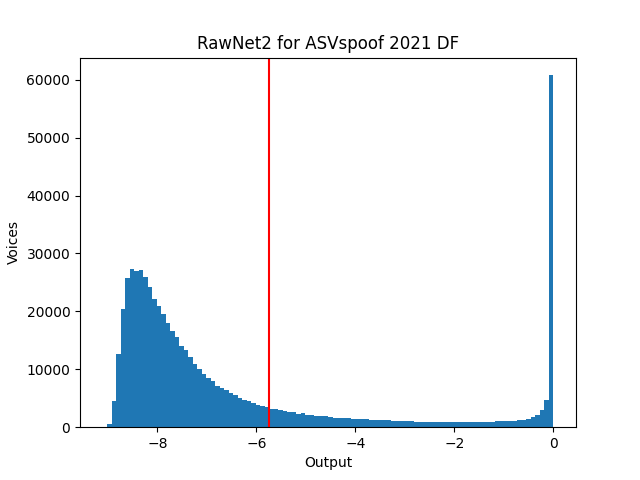
\includegraphics[width=\linewidth]{figures/rawnet2_asv.png} 
        \subcaption{}
    \end{minipage}
    \begin{minipage}[b]{0.45\hsize}
        \centering
        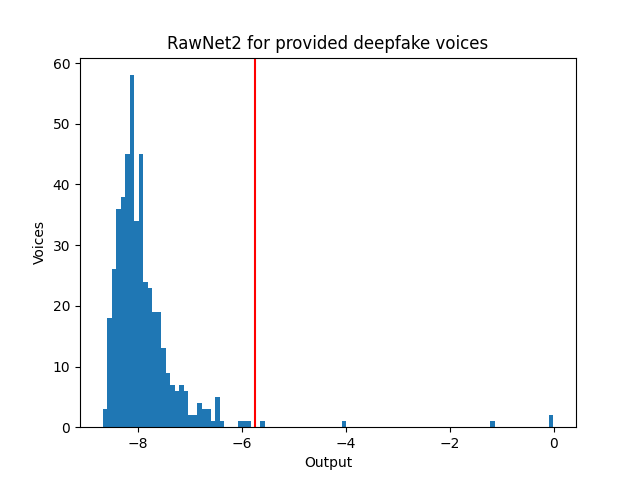
\includegraphics[width=\linewidth]{figures/rawnet2_prop.png}
        \subcaption{}
    \end{minipage}\\
    \begin{minipage}[b]{0.45\hsize}
        \centering
        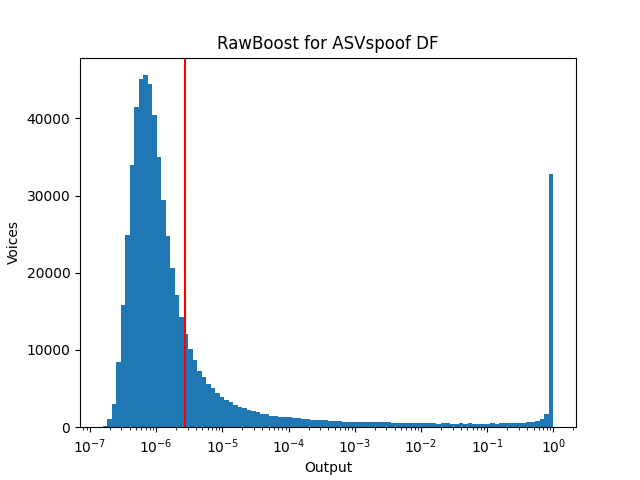
\includegraphics[width=\linewidth]{figures/rawboost_asv.png} 
        \subcaption{}
    \end{minipage}
    \begin{minipage}[b]{0.45\hsize}
        \centering
        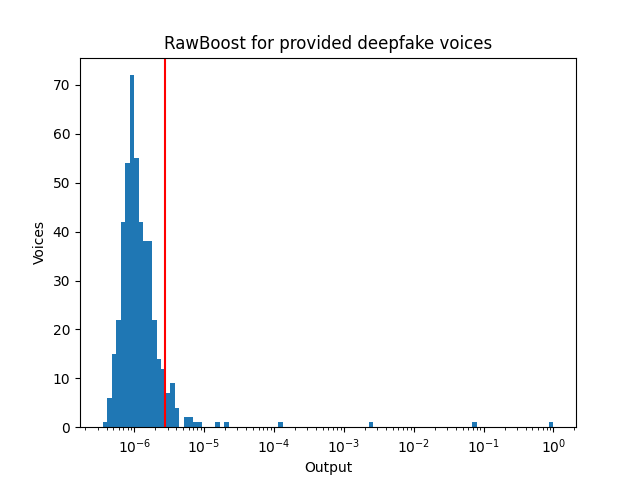
\includegraphics[width=\linewidth]{figures/rawboost_prop.png}
        \subcaption{}
    \end{minipage}
    \caption{モデルおよび使用データセット毎の出力値のヒストグラム。(a)ASVspoof2021DFに対するRawNet2、(b)提案偽情報データセットに対するRawNet2、(c)ASVspoofのRawBoost、(d)提供データセットのRawBoost。赤い線はASVspoofデータセット内のEERの状況に合わせた閾値を表す。}
    \label{fig:hist}
\end{figure}

また、RawNet2 の閾値が負の値であることに注意することが重要である。
これはLogSoftmax関数を適用するモデルの仕様の影響で、RawNet2の出力が常にゼロか負であるためである。
RawNet2の場合、その性能は\cite{yamagishi21_asvspoof}によるASVspoof 2021の記事で報告された結果と密接に一致する。
しかし、RawBoostに関しては、ASVspoof DFタスクでのパフォーマンスはRawNet2を下回る成績だった。
この傾向は、RawBoostが当初この特定のタスクのために設計されたものではなかったことに起因している可能性がある。
提案したデータセットからの出力値の適用を標準化するために、ASVspoof DFデータセットのEERから導き出した閾値を採用した。
このアプローチにより、異なるモデルやデータセット間で一貫性のある比較ができた。

表5にモデルの出力値を示す。
両モデルに共通する特徴は、出力値が音声に関連する疑いのレベルを反映していることである。
ASVspoof データセットの結果に基づき、ASVspoof データセットの EER で設定された閾値を超える値は、偽音声が疑われると本研究の実験では解釈する。
\cref{fig:hist}に示すように、ASVspoof データセットと比較すると、本研究の提供する音声は、偽音声として検出された割合が大幅に低下している。
この結果は、当社のデータセットが主に本物の音声で構成され、本物の音声は 1 つしか含まれていないことを考えると、重大な懸念事項である。
同様の傾向は、\cref{tab:preOut} の平均値と中央値を調べたときにも明らかであり、本研究が提供した音声の平均値と中央値は、ASVspoof 2021 DF タスクで観察された値よりも著しく小さい。
さらなる分析として、\cref{tab:greater}に出力が閾値を超えた偽音声の数を示す。
ASVspoofデータセットが閾値を設定し、出力値がこの閾値を超えた場合、その音声はDeepFakeとして識別されます。
RawNet2では5つの音声が偽音声として検出され、RawBoostでは32の音声が偽として検出された。
ただし、RawBoost は EER が低いため、結果の信頼性には疑問が残ることに留意が必要である。
この結果はどちらのモデルも、提供されたデータセットの全サンプルの 10\%未満しか偽音声として識別していないことを示す。
さらに、生成された音声を聴いたところ、明らかな偽音声として判別できるような目立ったアーティファクトや不自然な点は確認できなかった。
まとめると、どちらのモデルも入力音声を偽音声ではなく本物であると判断していた。


\section{本実験: 発話内容考慮による検出性能改善の検証}\label{sec:cnt_main}
本実験では、波形と発話内容を考慮して、新たに提案したフレームワークを検証した。
環境は、\ref{tab:env}が示すように、予備実験と同じ条件である。

\subsection{データセット}
本実験では、提案モデルにおいて、事実と偽の主張を伝える合成音声を含む別のデータセットを作成した。
この新しいデータセットは二値ラベルを採用し、合成音声を「事実」と「偽情報」の2クラスに分類する。
今回の文脈では、「事実」(``factual'')ラベルは事実を報じるニュースを伝える合成音声に割り当てられ、偽情報(``misinformation'')ラベルは偽情報を広める合成音声に該当する。
この2ラベルはMuMiN内での記載ラベル名に由来するものである。
本来\cref{ch:background}の通り``misinformation'' は誤報という定義に該当するが、MuMiNが保有する該当投稿の殆どが偽情報の定義にも該当するため、本研究では偽情報として扱う。
予備実験と本実験の顕著な違いの一つは、データセット内の事実と偽の主張の比率である。MuMiN-largeデータセットでは、英語の投稿8,013件を保有する。
しかしながら、事実を示す投稿は357件にとどまる。
この不均衡に対処するため、偽情報の数を意図的に減らし、事実の主張の量に近づけた。
全投稿数は723で、357の事実投稿と365の偽情報投稿である。
また、音声生成のための前処理として、すべての投稿からURLと絵文字を削除した。
本実験で使用した合成音声は、VITSモデルを利用し、予備実験と同じ条件でデータセットから取得した。
実験と評価を容易にするため、このデータセットをトレーニングセット、検証セット、テストセットに0.7/0.1/0.2の割合で分割し、学習およびテストを行った。

\subsection{実験内容}
この実験では、主張の信憑性を評価する要素の重要性を調査した。
その実現に向け、波形と音声コンテンツの両方を考慮する新しいフレームワークを評価した。
さらに、実験に必要な事実と捏造の主張に関連する合成音声を含むデータセットを導入した。

提案するフレームワークモデルの波形セクションでは、RawNet2を採用した。
モデルの設定を維持したまま、微調整なしで音声波形データを入力した。
その後、出力を0から1の範囲で正規化し、波形の疑わしさを表現した。
発話内容評価では、MuMiNデータセットから取得した投稿の埋め込みを利用した。
学習データセットの埋め込みに対してXGBoost分類器を訓練した。
最後に、提案するフレームワークの波形とコンテンツの両コンポーネントからの出力の平均を計算した。
最終出力は音声に関連する疑わしさの度合いを示している。
EERと正確性(Accuracy)に基づき、提案フレームワークモデルを波形のみ・コンテンツのみのモデルを含む単一ユニットモデルと比較した。 
また、ASVspoof 2019のLAセットでRawNet2の性能を確認し、このモデルが従来の手法で偽音声を正確に検出できる点を証明することを意図した。
EERを使用したのは、これがASVspoof 2021 DFの評価指標であったためである。
MuMiN+VITSによる音声セットやASVspoof 2019 LAセットの結果と比較するためにAccuracyを採用した。
これは、ASVspoof 2019 LAセットには事実のニューステキストしか含まれていないためである。
具体的には、EERの算出に必要な値であるTrue PositiveとFalse Negativeが不足しているため、コンテンツのみではASVspoofデータセットのEERを得ることができない。
そのため、別の指標であるAccuracyを設定した。

また、本実験ではSSL Anti-spoofingのMuMiN+VITSデータセットに対するパフォーマンスも確認した。
このモデルは、ASVspoof 2021 DF post-challenge \cite{10155166}の参加者の中で、最高のパフォーマンスを発揮していたことから、本実験で採用した。

\subsection{結果}\label{sec:cnt_res}
本実験では、モデルが偽情報を主張する合成音声を識別できるかどうかを検証した。
この本実験の結果を\ref{tab:result}に示す。
波形のみのモデルの場合、EER は44\%で、accuracyは50\%に近く、ランダム選択に近い結果を示した。
この結果は、偽音声を波形のみの観点から検出するモデルの能力が限定的であることを浮き彫りにしている。
一方で、本研究が提案する波形と内容を考慮したモデルが最も優れていることが示された。

また、ASVspoof 2019 LAセットに対してRawNet2が正確に分類された点も確認した。
この結果はTakらの報告 \cite{9414234}を支持するものである。
SSL anti-spoofingの結果は、ASVspoofの結果において、他のモデルからの改善を示している。
この結果もASVspoof 2021の報告 \cite{10155166}を支持するものである。
しかし、MuMiN+VITSのデータセットにおけるEERは54\%であり、他波形単独手法と同様にまだ改善の余地がある。
この部分からも、波形のみで偽情報を話す偽音声を検出することは、最新の音声生成モデルでは不十分であることが示唆される。
また、これら2つのデータセットの平均値から、SSL anti-spoofingを含む比較モデルの中で、提案手法が最も精度の高い性能を示した。
この結果は、提案フレームワークは実際のSNS上での運用において最新の音声生成モデルと効果的に対応できることを示唆している。

\begin{landscape}
\begin{table}[p]
    \caption{事実に基づく情報と、事実と異なる偽情報を話す合成音声を真偽分類した結果。(*)は、データセットに偽情報記事が含まれていないため、計算不可能な値であることを示す。}
    \centering
    \begin{tabular}{lcc|ccc}\hline
         & \multicolumn{2}{c}{等価エラー率 [\%]} & \multicolumn{3}{c}{accuracy [\%]}\\
       モデル形式 & MuMiN + VITS & ASVspoof 2019 LA & MuMiN & ASVspoof & 平均\\\hline\hline
       波形のみ(RawNet2) & 44.6 & 5.6 & 52.7 & 99.7 & 76.2\\
       波形のみ(SSL anti-spoofing) & 54.1 & 2.9 & 46.3 & 99.8 & 73.1\\\hline
       内容のみ(埋め込み+XGBoost) & 32.4 & \multirow{2}{*}{N/A*} & 86.8 & 11.5 & 49.2\\
       提案手法: 波形+内容 & 17.6 & & 81.7 & 81.6 & 81.7 \\\hline
    \end{tabular}
    \label{tab:result}
\end{table}
\end{landscape}

\section{考察}\label{sec:cnt_evl}
\subsection{音声合成と検出の発展速度差}
予備実験の\cref{tab:preOut}によると、音声生成の進歩に検出が追い付いていない点が重要な問題として浮上している。
ASVspoofでベースラインとして提供されたRawNet2は、RawBoostと同様に、最新のText-To-Speech(TTS)で合成された音声を正しく偽として検出できなかった。
この結果は、2019年以前のTTSとVCモデルを組み込んだデータセットで訓練されたモデルは、2020年以降に開発されたモデルに対応できないことを意味する。
注目すべきは、この性能低下はASVspoof 2021の報告 \cite{yamagishi21_asvspoof}で以前から認められていたことでもある。
一方で本研究は、2021年以降の方法に特化した音声合成の結果を提供するものであり、その間に大きな合成側の前進がある。
偽音声合成側の進歩が速いため、新しい波形分析方式による偽音声検出手法が提案されてから、良好な検出成績を長い期間提供できない可能性が考えられる。

本実験の結果、\cref{tab:result}の各データセットの性能評価において、提案手法が最も優れていることが示された。
本実験は、発話内容の一部を考慮することによる改善点を確認することを目的としている。 
したがって、提案スコアは波形と内容において個々のモデルよりも優れており、この結果は我々のコンセプトの効果を証明している。

\subsection{提案手法の改善点}
我々の提案するフレームワークモデルは、現実のシナリオに適用した場合、顕著な改善を示している。
具体的には、SNS上に投稿された対象音声を我々のモデルに展開するシナリオを想定している。
この文脈では、投稿埋め込みを直接利用できないという課題に直面することに注意しなければならない。
この制限を克服するためには、音声認識モデルを採用して音声コンテンツをテキストに書き起こす必要がある。
最終的には、入力コンテンツが波形データのみで構成されている場合でも、
本研究の形式が効果的に音声を正確に分類できるようにする必要がある。

さらに、本人が偽情報を読む場合も想定し、合成音声と人間が録音した音声の両方を包含する追加データセットを作成する必要がある。
本稿では、提案モデルの偽の主張を検出する能力を評価することを主目的としたため、録音された音声を取り込まなかった。
本研究では今後録音された声と合成された声、そして事実と偽の内容という2つの観点を考慮した4クラス分類を含む別の実験も考えられる。
\cleardoublepage
\chapter{考察}
\label{ch:discussion}
本章では、本研究を実社会へ適用する際に想定される効果及び課題について記述する。

\section{多様化する媒体への対応}
\cref{ch:gen_com}では、記事に予想されるコメントを生成することで検出を補助するモデルを提案した。
本モデルの利点として、他の媒体への拡張が容易である点が挙げられる。
コメントはどの媒体の情報に対して共通して自然言語として使われるため、投稿とコメントがセットで提供されているデータセットがあれば、画像・動画・音声問わずどの形式の偽情報にも適用が可能となる。

\section{大規模言語モデルによる影響}
大規模言語モデル(LLM)の性質として、事実に基づかない情報を提供するハルシネーション(Hallucination)が指摘されている \cite{Alkaissi2023-bo}。
これはモデルの学習及び推論・改善において文章の自然さが優先され、事実に基づくかがあまり確認されていない点が理由として考えられる。

さらに、偽情報提供側がLLMを利用した意図的にミスリードを狙った投稿への対策も必要である。
\cref{ch:rel_res}の通り、既にThai Leら \cite{9338282}によってコメントを考慮した検出モデルを誤認させる手法が提案されている。
よって、学習において投稿されたコメントが実際に利用者によって書かれたか考慮する必要が生じている。

これらの問題点は知識ベースをLLMに組み込むことで改善を目指した研究も紹介されている \cite{10.1145/3512467}。
しかしながら、LLMの発展によって人間による文章かAIによる文章か見分けが難しくなっている点も指摘されている \cite{Elkhatat2023,chen2023can}点から、
自然言語処理における生成文章検出タスクのさらなる発展が求められている。

\section{動画への個別対応}
\cref{ch:introduction}の通り、本研究では偽情報動画の流布が他媒体と比べて多くないとして対象から除外した。
一方で、動画生成技術も発展を続けておりSora \cite{videoworldsimulators2024}に代表されるような高精細な映像も生成可能になりつつある。
開発したOpenAIは安全対策としてC2PAと呼ばれる電子透かし \cite{C2PA}の導入や、
生成プロンプトの内容によって偽情報生成を防止するシステム \cite{AI_2023}の適用を約束している \cite{AI_2024}。

しかしながら動画に限らず生成AI全体において、既存の防止システムの突破(jailbreak)を目的とした研究が幾つかある \cite{NEURIPS2023_fd661313,shayegani2024jailbreak}ため、
偽情報生成・検出と同様いたちごっこの様相を呈している。
また、今後ローカル環境での生成が可能になった場合は防止システムによる抑止が難しい点からも、動画生成側の技術発展による偽動画による偽情報投稿が今後急激に増える点が予想される。
検出においては、データセット作成において生成例が必要である点から実際の動画生成モデルの提供を待たなければならないが、今後個別対応が必要と考える。

\section{プラットフォームへの依存}
SNS上の検出を目指した場合、SNSプラットフォームへの依存は不可避の要素である。
しかしながら、プラットフォーム側の姿勢の変化により研究の障壁が大幅に変動する問題がある。
特に$\mathbb{X}$(旧Twitter)はイーロン・マスク氏による買収前は研究目的であれば投稿の取得が無償で行えたものの、
本論文執筆現在は月額課金として1万投稿/月に100米ドル、100万投稿/月に5000米ドル \cite{Twitter}と高額な料金が必要である。
このようなプラットフォーム側の姿勢によって、偽情報対策を目指す活動が抑制される可能性を危惧している。

\cleardoublepage
\chapter{おわりに}\label{ch:conclusion}
%かつてはマスメディアが中心となって情報を広めていたため、組織内での精査によって発信される情報の質はある程度担保されていた。
%その中で
ソーシャル・ネットワーキング・サービス(SNS)は誰もが様々な情報を発信できるだけではなく、見かけた情報を不特定多数へ共有できることで、広く利用者に受け入れられた。
しかしながら、投稿された情報が短い時間によって広く拡散される点から、意図的に事実と異なるように作成された偽情報も広まりやすくなった。

既存手法が抱える問題点として、情報の媒体変化への対応に難しい点が挙げられる。
%例えば自然言語で書かれた偽情報そのものの内容のみで学習した場合、
特に近年は動画や音声といった新しい媒体を主とするSNSも若年層を中心に使われている一方で、
既存の自然言語で書かれた偽情報を想定したモデルはそのような媒体には対応できない。
またもう1つの問題点として、とりわけ音声は任意の人物の音声を短い時間のサンプルで忠実に再現できる一方で、
既存手法による対策は音声波形のみを対象としており、生成側の発展に追いついていない点も挙げられる。
本研究は、それぞれの問題に対応する新たな手法を提案する。

媒体変化に頑強な手法として、あらゆる形式に対して共通して自然言語の形をとるコメントを活用した。
既存手法では偽情報に対してコメントが批判的になるため、コメントの活用が検出に有用であることが示されていた。
一方で拡散の初期段階で検出を目指す場合、使用できるコメントの数は制限される。
本研究では検出を補助するために、コメントの生成を行った。
実装にあたって、架空の記事を生成する手法を改変し、実際に投稿された記事と3件のコメントから生成の学習を行った。
実験では、まず実際に投稿された記事と2件の投稿済みコメントから学習済生成モデルがコメントを追加した。
続いて、別の偽情報検出モデルにこれらの情報を入力し、偽情報であるかの判断を行った。
検出の結果は、コメントそのものの有用性の確認として記事本文のみで検出を行った場合と、コメント生成の有用性の確認として記事と投稿済コメント2件で検出を行った場合と比較した。
提案手法の偽情報全体の件数のうち実際に検出できた割合である再現率(Recall)は0.695と全体で最も高い結果を示した。
%一方で偽情報と検出した中で実際に偽情報だった割合を示す適合率(Precision)には改善の余地を残した。
また投稿済みコメントのみで分類したときに事実に基づく情報と誤って判断した件数のうち、生成コメントの追加によって偽情報と正しく判断できた割合が48\%と、コメント生成の効果を確認した。
この手法はどの媒体に対しても必ず自然言語の形を取るコメントの生成という新しい形式の真偽判断材料を提供する。
これはSNSプラットフォームの変化に頑強であるため、長い期間利用者や検出モデルに対して真偽を判断する新たな情報を与えられる。

音声による偽情報対策として、発話された内容も考慮した偽情報の検出も目指した。
これは既存手法にはみられない新しい視点として、SNS上で投稿された音声による偽情報の検出に必要な発話内容の考慮を取り入れている。
具体的には、音声波形の分析を行う既存手法に加えて、文章埋め込みとして話された内容から得た情報によって信憑性を評価する部分から構成している。
実験では、実際にSNSに投稿された偽情報文章から直近に提案された音声合成手法によって得た音声データセットを使用した。
音声波形のみを考慮した既存手法では、他人受入率と本人拒否率が一致するよう閾値を調整した際のエラー率である等価エラー率が50.7\%を示し、無作為に真偽を判断した場合に近しい結果を示した。
一方で提案手法では等価エラー率が17.6\%まで改善し、提案する視点の有用性が示された。
この手法は現在検出が難しい疑わしい主張を行う音声に対して音声波形と発話内容から信憑性を評価できるため、
SNS上に投稿された偽情報音声を正確に検出できる。

今後SNSの安全性を維持するためには、共有される情報の媒体の多様化に対応しなければならない。
本研究が提案する2つの手法は、それぞれ媒体の多様化に頑強であることと、現状さらなる対策が必要な媒体である音声へ特化しているという特長がある。



%======  謝辞      ======================================================%
\cleardoublepage
\chapter*{謝辞}

%======  参考文献  ======================================================%
\cleardoublepage
\bibliography{references}
\bibliographystyle{junsrt}
%======  付録  ======================================================%
%\cleardoublepage
%\input{furoku}
%======  研究業績  ======================================================%
\cleardoublepage
\chapter*{研究業績}
\section{査読付き学術論文}
\begin{enumerate}
    \item \underline{Yuta Yanagi}, Ryohei Orihara, Yasuyuki Tahara, Yuichi Sei, Tanel Alume, Akihoko Ohsuga: The Proposal of Countermeasures for DeepFake Voices on Social Media Considering Waveform and Text Embedding, Annals of Emerging Technologies in Computing, Vol. 8, Issue 2, pp.15-31, 2024.
\end{enumerate}

\section{査読付き国際会議}
\begin{enumerate}
    \item \underline{Yuta Yanagi}, Ryohei Orihara, Yasuyuki Tahara, Yuichi Sei, Tanel Alume and Akihiko Ohsuga: Inspection of The Classifying Performance of The Deepfake Voices by The Latest Text-to-Speech Models, 2nd Interdisciplinary Conference on Mechanics, Computers and Electrics (ICMECE), pp. 330–335, 2023.
    \item \underline{Yuta Yanagi}, Ryohei Orihara, Yuichi Sei, Yasuyuki Tahara and Akihiko Ohsuga: Fake News Detection with Generated Comments for News Articles, 24th IEEE International Conference on Intelligent Engineering Systems (INES), pp.85–90, 2020.
\end{enumerate}

\section{国内発表}
\begin{enumerate}
    \item \underline{柳 裕太},折原 良平,田原 康之,清 雄一,大須賀 昭彦, 偽情報の早期自動検出に向けたニュース 記事コメント生成モデルの提案, 17 回テキストアナリティクス・シンポジウム, 2021.
    \item \underline{柳 裕太}, 折原 良平, 清 雄一, 田原 康之, 大須賀 昭彦, 記事コメント生成による偽情報の早期検出,情報処理学会第 200 回知能システム研究発表会, SMASH20 (Symposium on Multi Agent Systems for Harmonization 2020) Summer Symposium, 2020.
    \item \underline{柳 裕太},清 雄一,田原 康之,大須賀 昭彦:画像付き偽情報とジョークニュースの検出・分類に向けた機械学習モデルの検討, マルチエージェントと協調計算(MACC)研究会, 2019. 
\end{enumerate}

%========================================================================%
\end{document}
